\documentclass[12pt]{report}
\usepackage{graphicx} % Required for inserting images
\linespread{1.2}

\usepackage{enumitem}
\usepackage{amsmath}
\usepackage{listings}
\usepackage[dvipsnames]{xcolor}
\usepackage{tikz}
\usepackage{mathrsfs}
\usetikzlibrary{positioning}
\usepackage[breakable]{tcolorbox}
\usepackage{colortbl}
\appto{\bibsetup}{\raggedright}

\definecolor{lightgray}{rgb}{0.95, 0.95, 0.95}

\tikzstyle{mybox} = [draw=RoyalBlue, fill=RoyalBlue!5, ultra thick, rectangle, rounded corners, inner sep=10pt, inner ysep=15pt, text width=0.90\textwidth, align=left] 
\tikzstyle{boxtitle} = [fill=RoyalBlue, text=SkyBlue!30, ultra thick, rectangle, rounded corners, inner sep=10pt, inner ysep=8pt, text width=0.90\textwidth]

\newcommand{\BoxDef}[2]{%
\vspace*{10px}
\noindent

\begin{center}
\begin{tikzpicture}
    \node[mybox](box){\rule{0pt}{30pt}\ignorespaces#2\unskip};
    \node[boxtitle, anchor=north west] at (box.north west) {\textbf{#1}};
\end{tikzpicture}
\end{center}
}

\usepackage[hidelinks]{hyperref}
\usepackage{amssymb}
\usepackage{amsmath}
\usepackage{bm}
\usepackage[top=2.5cm, bottom=2.5cm, left=3cm, right=3cm, centering]{geometry}
\usepackage{algorithm}
\usepackage{algpseudocode}

\begin{document}

\begin{titlepage}
\hrule
\vspace{15pt}
\begin{center}
    \Huge{\textbf{\Huge \textbf{Computational Models For Complex Systems (6 cfu) 23-24}} \\ Notes}\\
\end{center}
\vspace{15pt}
\hrule
\vfill
\hrule
\begin{center}
    \Large University of Pisa \\ M.Sc. in Computer Science
\end{center}
\end{titlepage}

\tableofcontents
\chapter{Introduction}

\section{What is a Model of a System?}
A model is a simplified and approximate representation of a system, that allows reasoning on the systems properties. \textbf{So we construct models in order to understand some aspect of that system}. We include in the model only the aspect of the system that we consider essential, omitting details that would only complicate the analysis.

\subsection{Understanding the model}
After designing our model, then in order to acquire new knowledge, we have to \textbf{analyze the model} (like a child play with a toy to understand what it does), then we have to apply some \textbf{reasoning} regarding the result given during the analysis. 

\subsection{Errors}
All the three steps listed above (Modelling, Analysis, and Reasoning), \textbf{can be sources of errors}. The model can be too abstract; the analysis can be too inaccurate; or the interpretation itself could be wrong. \textbf{Recall that the result that you get are showing you only something about the real system, you need to generalise what the result means.}

\subsection{Examples of Models}

\subsubsection{Planimetries/project and scale models}
In architecture planimetries and scale models are used to assest structural properties at design time, in order to evaluate the result in advance.

\subsubsection{Life Science}
In biology rats (in-vivo model) or a cell colture (in-vitro model) are used as model for the human being. 

\subsubsection{In Silico Models}
In biology there are also computer-based techniques are usually faster and cheaper than in vivo e in vitro models. They simulate the interaction between proteins.

\subsection{Mathematical Models}
Mathematics provides tools for building abstract models of almost everything like \textbf{geometry} for Architecture or \textbf{differential equations} for Weather. Mathematical models have two advantages:

\begin{itemize}

\item They are formal model specification languages, meaning it is not an ambiguous model.

\item there are a lot of analytical and numerical methods to analyze model of this type.

\end{itemize}

\subsection{Computational Models}
Computational Models is similar to Mathematical Models. A Computational Model is a mathematical representation of a dynamical system (systems which evolves over time) taking a computer-executable form.
\par in Computational Model we are restricting the class of systems of interest to dynamical systems (systems which evolve over time). 

\subsubsection{Dynamical Systems}
Dynamical systems are systems that \textbf{evolve} by changing their state over time. Typically the state of a dynamical system is represented by a finite set of variables called \textbf{state variables}. In addition we will have some some law/rules/equations that describe how the state variables will vary over time. Our focus will be in prediction or analyze how the state of a dynamic system changes.
\par There are different types of dynamical systems depending on how the values of the variables change in either a discrete or a continuous way (or both).
\par \textbf{Note: time can be interpreted as a discrete or continuous entity}. 

\begin{figure}[h]
    \centering
    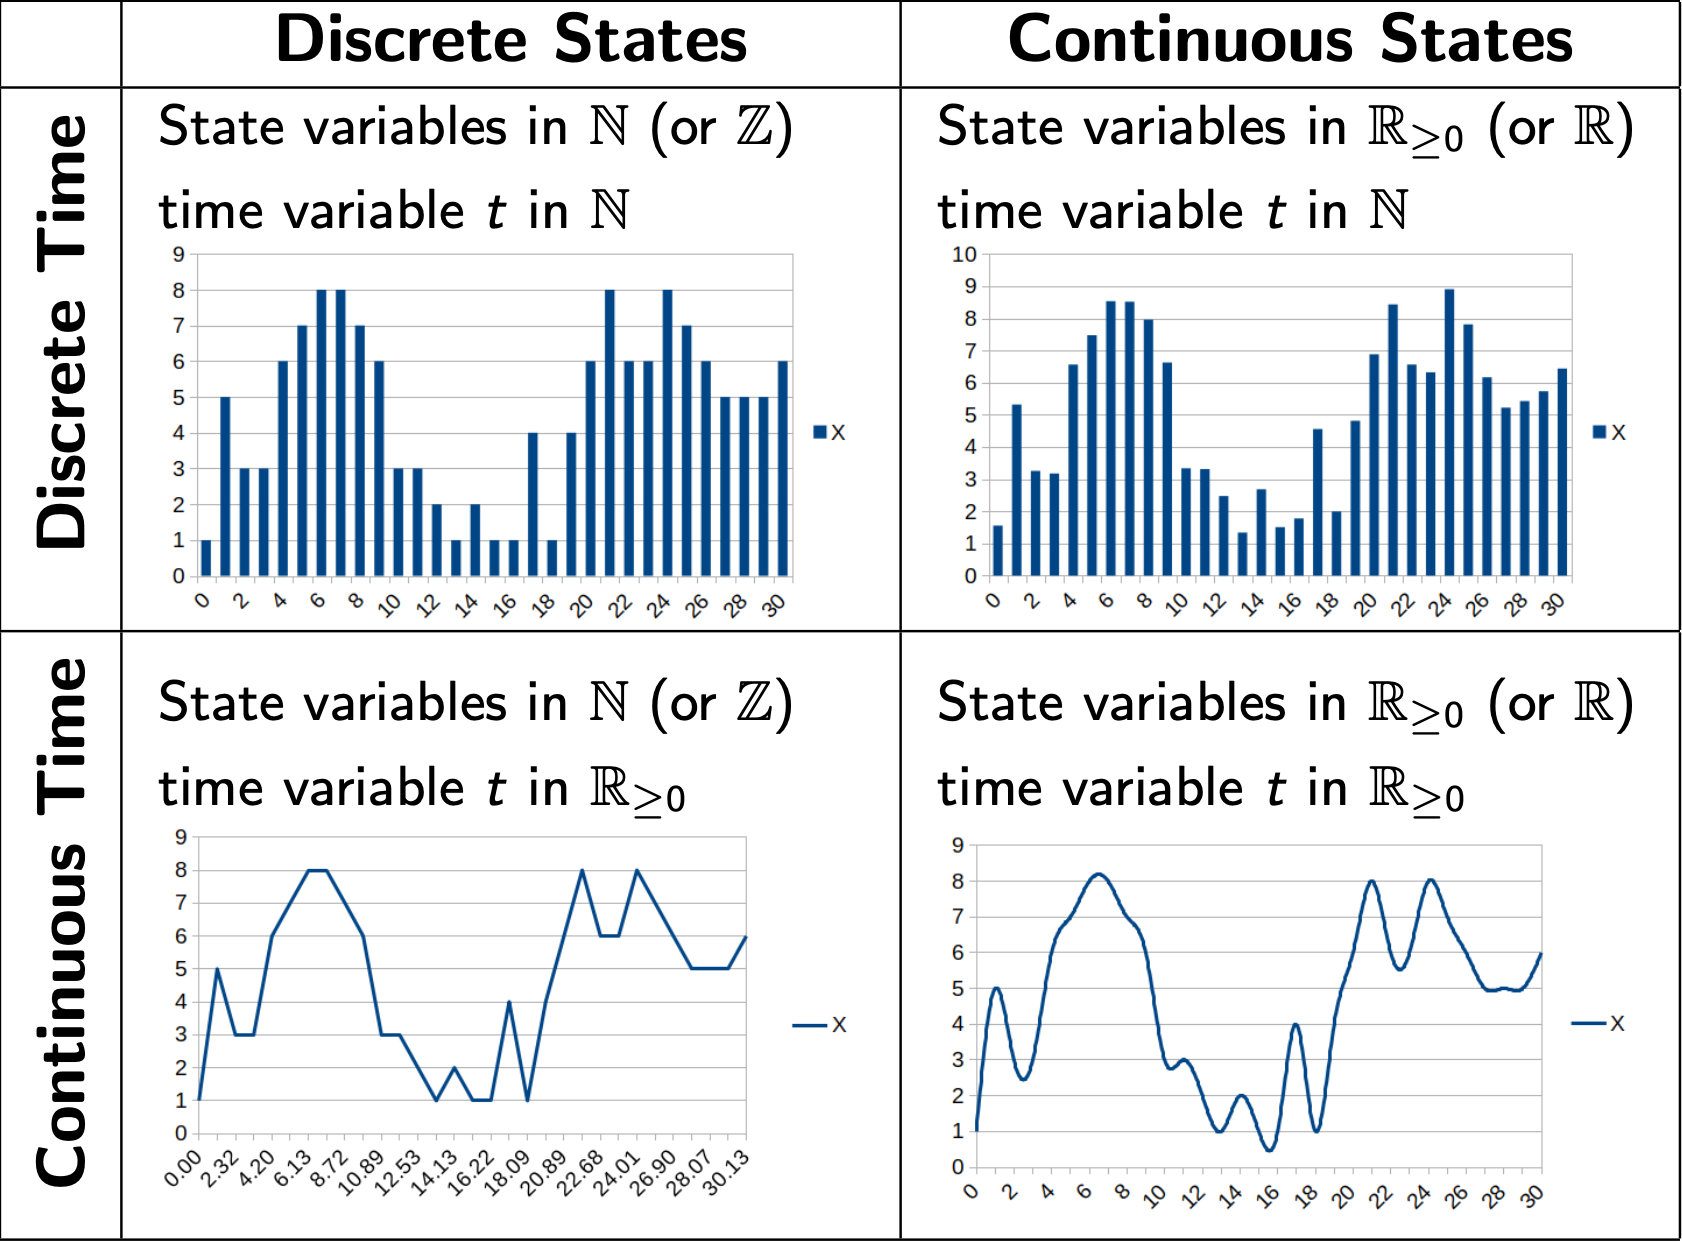
\includegraphics[width=0.8\textwidth]{Images/01-Introduction/states.png}
    \caption{All possible types of dynamical systems.}
\end{figure}

\subsection{Case of application}
What kind of analysis could we do with models of dynamical systems?

\begin{itemize}
    \item \textbf{Reachability of states:} predict the future state of the dynamical system.

    \item \textbf{Behavioral patterns:} the sequence of state that I pass through over time.

    \item \textbf{Effects of perturbations/ control strategies:} once I have a model of a system and I can simulate it, I can try to study how it will behave if I modify it.
\end{itemize}

\subsection{How to build a computational models?}
There are multiple ways

\subsubsection{The Data-driven way}
The Data-driven way (e.g. machine learning) consist in starting from the data of the system you want to model and then you apply some machine learning/optimization/whatever method to infer the model automatically. The generated model takes a form suitable for the inference method used. If enough data in available, it often works very well (good predictions), however inferred models are often very difficult to be interpreted (meaning that we can do good prediction, but we can't explain why they are correct).

\subsubsection{The Knowledge-driven way} (also called mechanistic models) consist in trying to reproduce through a mathematical model the internal mechanism of the system in order to reproduce the behaviour and to understand the internals of the systems. It requires limited data, but a good knowledge about the system functioning. Model construction usually requires some effort, and often predictions suffer from approximations but the method generated works also when few data are available; the model is interpretable: it contributes to understanding why a system behaves as observed; modelling allows validation hypotheses on the system functioning.

\section{What is a complex system?}
A complex system is a system consisting of many components (typically with a simple individual behaviours) interacting with each other, from these interaction emerges the global behaviour of the system.

\subsubsection{Complex Networks}
Complex Networks is a graph with complex structural properties. The dynamics of these networks and its evolution is a field of study (complex networks theory).

\subsection{Modeling notations for complex systems}
Many modeling languages are available for complex systems:

\begin{itemize}
    \item \textbf{mathematics:} Recurrence relations and differential equations.

    \item \textbf{concurrency theory:} we can apply methods seen in the study of concurrent system like Petri nets. Rewrite rules (Multiset rewriting) that describe the different events that happens in a complex systems as rules.

    \item \textbf{artificial life:} approaches proposed to try to reproduce behaviour seen in life. Cellular automata that describe the population as a grid; agents based model in which you explicit as an agent (e.g. an algorithm or set of functions/procedures) and then you can put the agent in a virtual environment to see how they behave together. 
\end{itemize}

\section{Analyze the model}
Modeling languages allow the modeler to express relationships between the state variables of a system and the rules/laws that determine the change of their values over time. The dynamics (or behaviour) of the systems (the actual sequences of states reached by the system over time) can be computed according to the semantics of the modeling language.

\section{Analyze the behaviour}
After the model has been specified, then there are multiple way to analyze the model. 

\subsection{Simulation}
You can try to apply some simulation algorithm in order to try to execute that model to have a possible evolution of the system. If the system is deterministic you have only one possible evolution, instead if the system is stochastic-probabilistic you will repeat the simulation several time and get different behaviour of the system. \textbf{So simulations can give you only some possible behaviour, not all}. Instead of running simulations to construct some description of the overall behaviour of the systems, it can be done by using \textbf{transition systems}. 

\subsubsection{Transition system}
A transition system is a graph (possible infinite) that describe the possible behaviour of a system. A possible transition system is the \textit{Makov chain}

\subsection{Model Checking}
It is an approach that determine whether the whole transition system satisfies a given dynamical property.

\section{Modeling vs programming}
The approach that we will follow to analyze dynamical systems is similar to the approach used to analyze programs

\begin{figure}[h]
    \centering
    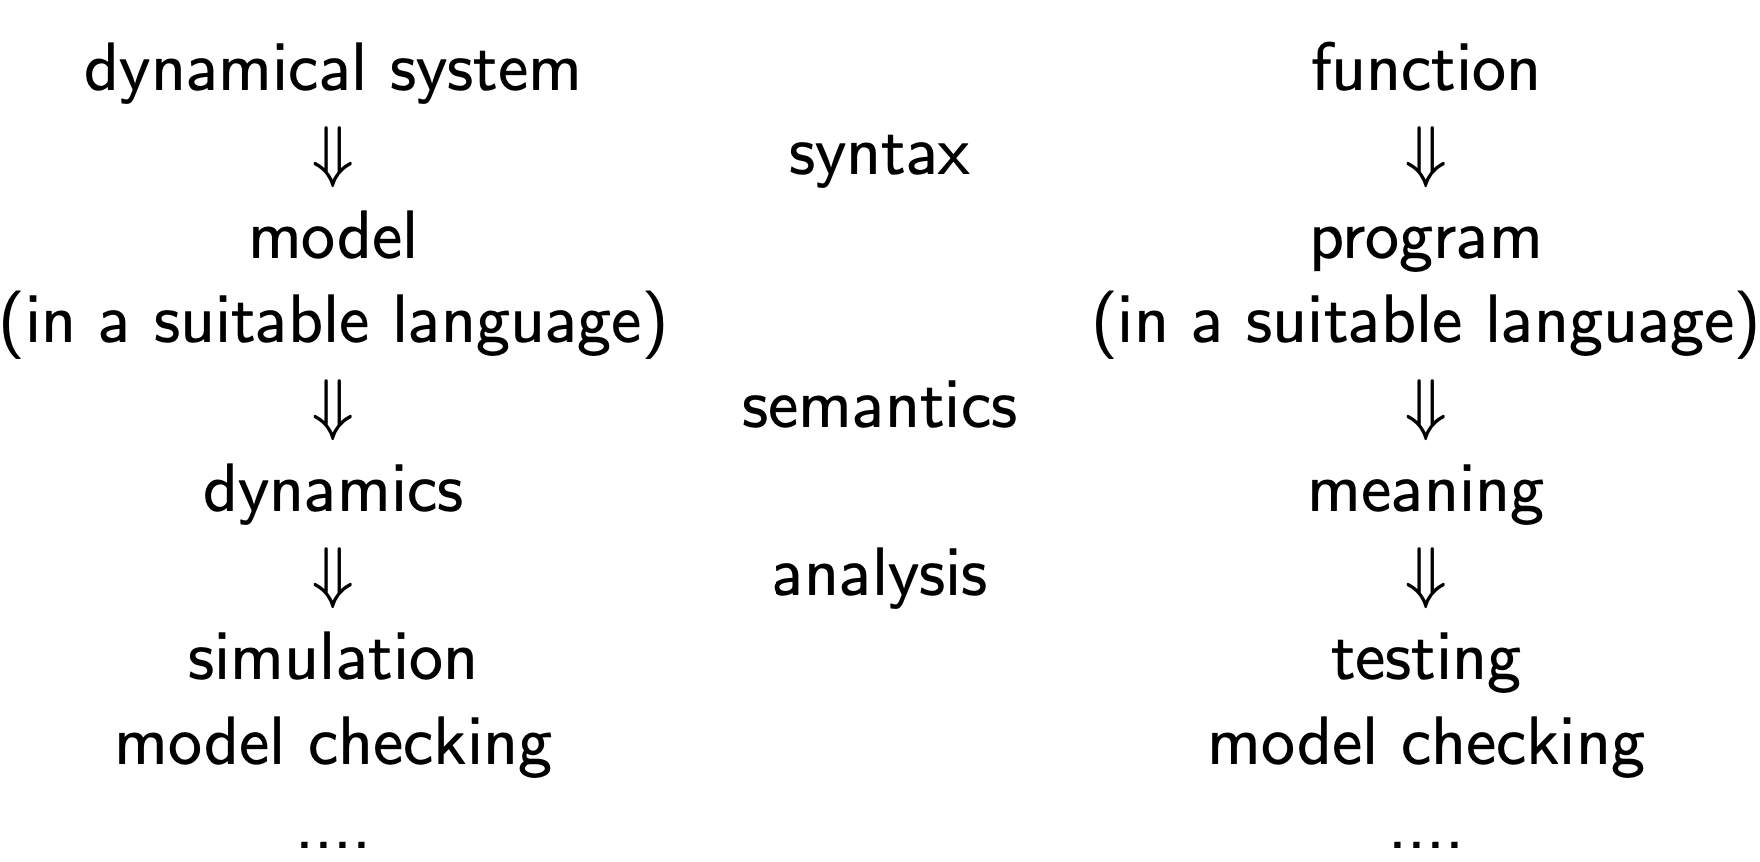
\includegraphics[width=0.9\textwidth]{Images/01-Introduction/model vs programming.png}
    \caption{Modeling vs programming.}
\end{figure}

\chapter{Discrete Dynamical Systems}
They are systems where the evolution is performed using discrete steps, in which the variables describing the state of the system are updated.

\section{Recurrence relations (Difference equations)}
Relations that tell you how from the current state of the discrete systems you obtain the next state of the systems, that is how from the original values the go to the new ones.
\par In this schema we will consider a generic system that is considered as a \textbf{population}(birth/death of individuals). Even the simplest form of interaction between individuals can lead to the emergence of \textbf{complex behaviors} (chaotic behavior) in the population. 

\section{Linear Birth Model}
The linear birth model is the simplest model describing a recurrence relation.
\par Given a population, each individual is \textbf{indistinguishable} from each other. We denote with \texttt{N(t)} the \textbf{density of some population} at a time \texttt{t}, that is the variable that describe the number of individuals that are part of the population at time \texttt{t}.
\par Given this description we want to predict what will happen to the density of the same population at a future time $t^{'} = t + \Delta{t}$ assuming that:

\begin{itemize}
    \item all individuals are indistinguishable from each other.
    
    \item there is enough food and space for every individual.
    
    \item each individual has $\lambda$ children every $\sigma$ time units.

    \item there is no death occurring in the interval $ [t, t + \Delta{t} )$.

    \item children do not start reproducing in the interval $ [t, t + \Delta{t} )$.
\end{itemize}

\begin{figure}[h]
    \centering
    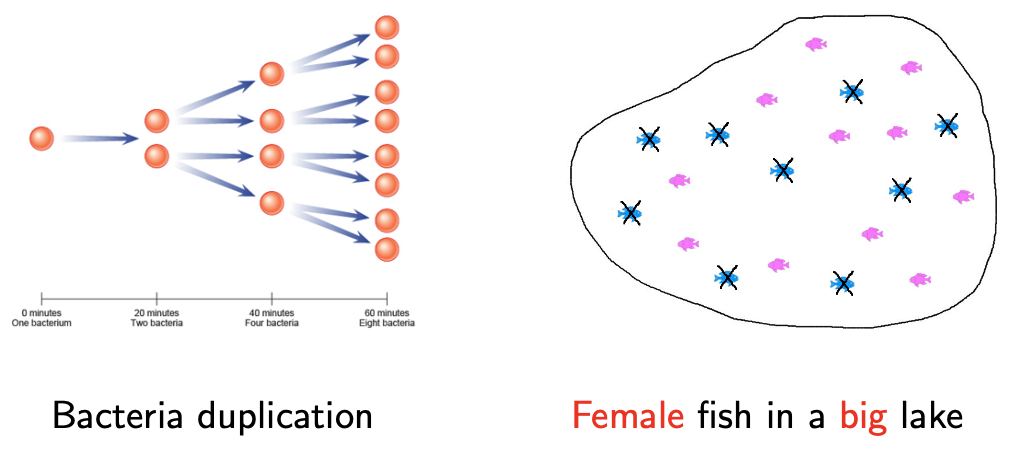
\includegraphics[width=0.8\textwidth]{Images/02-Discrete Dynamical Systems/Example_Linear_Birth_Model.png}
    \caption{Example of populations satisfying the assumption. In the bacteria example in order to assume
            the no children duplication we set $\Delta{t} \leq 20 minutes$} 
\end{figure}

\subsection{Describing the birth process as a relation}
The idea is that the size of the population at time $N(t + \Delta{t})$ will be $\geq$ than $N(t)$ since we assume \textbf{that there is no death occurring in the interval $ [t, t + \Delta{t}$]}. Additionally we know from our assumption that each \textit{adult} individual has $\lambda$ children every $\sigma$ time units.
\par Then, the number of individuals at time $t + \Delta{t}$ corresponds to the number of individuals at time $t$, plus the number of newborns at time $\Delta{t}$:

\begin{center}
    $N(t + \Delta{t}) = N(t) + \lambda{\frac{\Delta{t}}{\sigma}{N(t)}}$
\end{center}
if we group for $N(t)$ then the equation can be rewritten as follows:
\begin{center}
    $N(t + \Delta{t}) = N(t) * (1 + \lambda{\frac{\Delta{t}}{\sigma}}) $
\end{center}
    

\par Where $\frac{\Delta{t}}{\sigma}$ \textbf{describes the birth moments for every \textit{adult} individual in the interval $[t, t + \Delta{t}]$.}

\section{Constructing our algorithm}
Defined our equation \textbf{we can derive a discrete model from it}.
\par We choose a \textbf{time step} (discretization step) that describe an update of the population, in our case \textbf{the time necessary for a newborns to be considered an adult so that it can reproduce}, and we set it as $\Delta{t}$.
\par Instead of representing the equation fully we rewrite it using the \textbf{notation of sequence theory} by instead of using the actual value of the time $\Delta{t}$, we just count the steps. Thus we obtain:
\begin{center}
    $N_{t+1} = r_{d}N_{t}$
\end{center}
where $r$ stands for \textit{rate}; $d$ stands for \textit{discrete}; $r_{d}$ represents the \textbf{constant birth rate} s.t. $r_{d} = \lambda{\frac{\Delta{t}} {\sigma}}$.

\subsection{Defining the general term of our equation}
Given the recurrence relation we can \textit{sometimes} calculate the \textbf{general term}, that is the solution of the recurrence relation. In the case of our linear birth model it is a \textbf{non-recursive definition of $N_{t}$}.
\par To do so we first calculate the first terms of $N_{t}$: $N_{1}, N_{2}, N_{3}, ...$

\begin{center}
    \begin{itemize}[label={}]
        \item $N_{1} = r_{d}N_{0}$

        \item $N_{2} = r_{d}N_{1} = r^{2}_{d}N_{0}$

        \item $N_{3} = r_{d}N_{2} = r^{3}_{d}N_{0}$
    \end{itemize}
\end{center}

We notice how \textit{it seems} that $N_t = r^{t}_{d}N_{0}$, \textbf{but we have to prove it}.
To prove the formula, since we are in the realms of the natural numbers, we can use \textbf{mathematical induction}:

\begin{itemize}[label={}]
    
    \item \textbf{Base Case (t = 0):} $N_{0} = r^{0}_{d}N_{0}$ which is true.
    
    \item \textbf{Induction Case (t = k + 1):} we assume that the formula is correct for $t = 0$ to $t = k$ and check if it is true for $t = k + 1$. We know from assumption that $N_{k+1}$ will be a summation between the previous value for $t = k$ and the newborns in the current step. $N_{k+1} = r_{d}N{k}$ and we know from \textbf{induction hypothesis} that $N_{k} = r^{k}_{d}N_{0}$, thus we can rewrite $N_{k+1}$ as $N_{k+1} = r_{d}(r^{k}_{d}N_{0}) = r^{k+1}_{d}N_{0}$ proving the thesis.  
    
\end{itemize}

Now having the general term $N_{t} = r^{t}_{d}N_{0}$ we can compute the solution of our model.

\subsubsection{Phase portrait}
A way to represent recurrence relations graphically is through \textbf{phase portrait}. It consists in putting in the \textit{Cartesian plane}:
\begin{itemize}
    \item \textbf{x-axis}: $N_{t}$

    \item \textbf{y-axis}: $N_{t+1}$
\end{itemize}

Then in the plane we plot the recurrent relation. First you draw the bisector and you draw the recurrence relation as a function, then by starting from point $(N_{0}, N_{0})$ on the bisector, the other point can be obtained by \textit{"bouncing"} on the curve of the recurrence relation. \textbf{You can see how fast the quantity increases (or decreases) over time}.

\begin{figure}[h]
    \centering
    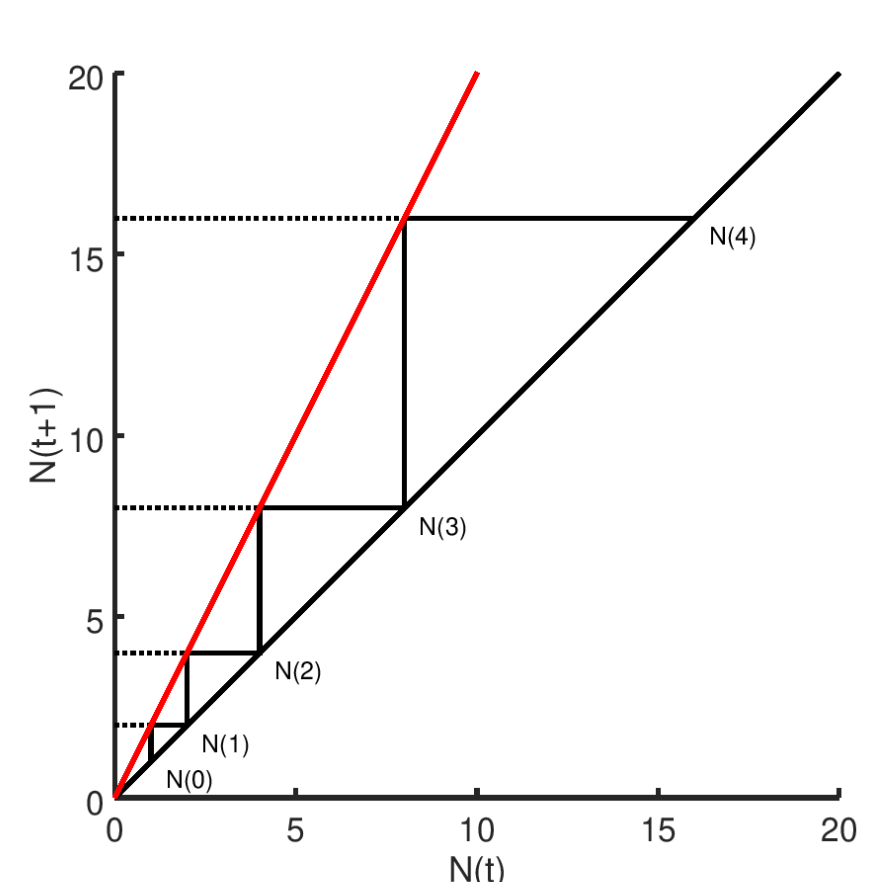
\includegraphics[width=0.5\textwidth]{Images/02-Discrete Dynamical Systems/phase_potrait.png}
    \caption{} 
\end{figure}

\begin{center}
    Above an example of phase portrait in our linear birth model. 
    \par In \textcolor{red}{red} we draw the recurrence equation $N_{t+1} = 2N_{t}$.
    in \textbf{black} the bisector $N_{t+1} = N_{t}$. 
\end{center}

\section{Introducing death in our model}
We complicate our recurrence relation by considering also deaths, so we are adding a negative term that decrease the number of individuals of our population over time. 
\par Assume that, a constant fraction $s_{d}$ \textbf{of adults that die in every time step} $\delta{t}$. Then our recurrence relation now is:
\begin{center}
    $N_{t+1} = r_{d}N_{t} - s_{d}N_{t}$
\end{center}

By grouping for $N_t$ we can rewrite the equation as:

\begin{center}
    $N_{t+1} = (r_{d} - s_{d})N_{t}$
\end{center}

\textbf{Note:} since the number of individuals which die cannot be greater than the whole population, then $ 0 \leq s_{d} \leq 1$

\par Since $r_{d}$ and $s_{d}$ are two constant, one positive and one negative, we can group them together in one single constant $\alpha_{d} = (r_{d} - s_{d})$. We call $\alpha_{d}$ the \textbf{net growth rate}, that is the rate where you discard the individuals who dies. We can rewrite our equations as:

\begin{center}
    $N_{t+1} = \alpha_{d}N_{t}$
\end{center}

The difference in respect of the previous case is that $\alpha_{d}$ will be in general greater than 0, but not necessarily greater than 1.

\subsubsection{General trend of our model}
There could be many possible cases depending on the value of the constant $\alpha_{d}$:

\begin{itemize}

    \item $\alpha_{d} > 1$: the overall behaviour of the population is the same as before, \textbf{since the population at every steps will increase}.

    \item $\alpha_{d} = 1$: the population remains constant, \textbf{since the number of newborns always is equal to the number of dead ones}.

    \item $\alpha_{d} < 1$: if for instance we assume we have less newborns than the death of old individuals, \textbf{then at every step the population reduces}.
    
\end{itemize}

\section{Introducing migration in our model}
Independently from the size of the population, \textbf{we assume a fixed number of individuals arrive in our region}. We only consider people that arrives, so we model the migration using a constant and positive parameter declared as $\beta$. 
\par Then our equation becomes:

\begin{center}
    $N_{t+1} = \alpha_{d}N_{t} + \beta$
\end{center}

with $\beta \geq 0 $ representing the number of individuals entering the population every $\Delta{t}$ time units.

\par By \textbf{mathematical induction} we can prove the general term is:

\begin{center}
    $N_{t} = \alpha^{t}_{d}N_{0} + \sum_{i=0}^{t-1}{a^{i}_{d}\beta}$
\end{center}

where $\sum_{i=0}^{t-1}{a^{i}_{d}\beta}$ accumulates the $\beta$ individuals that arrived in the previous step (from 0 to $t-1$) and the children produced by them at every step.

\subsection{Simulating the migration}
Having our general term, we can see what happens by varying $\alpha_{d}, N_{0}$ and $ \beta:$
\par \textbf{Case $\alpha_{d} > 1$}

\begin{figure}[h]
    \centering
    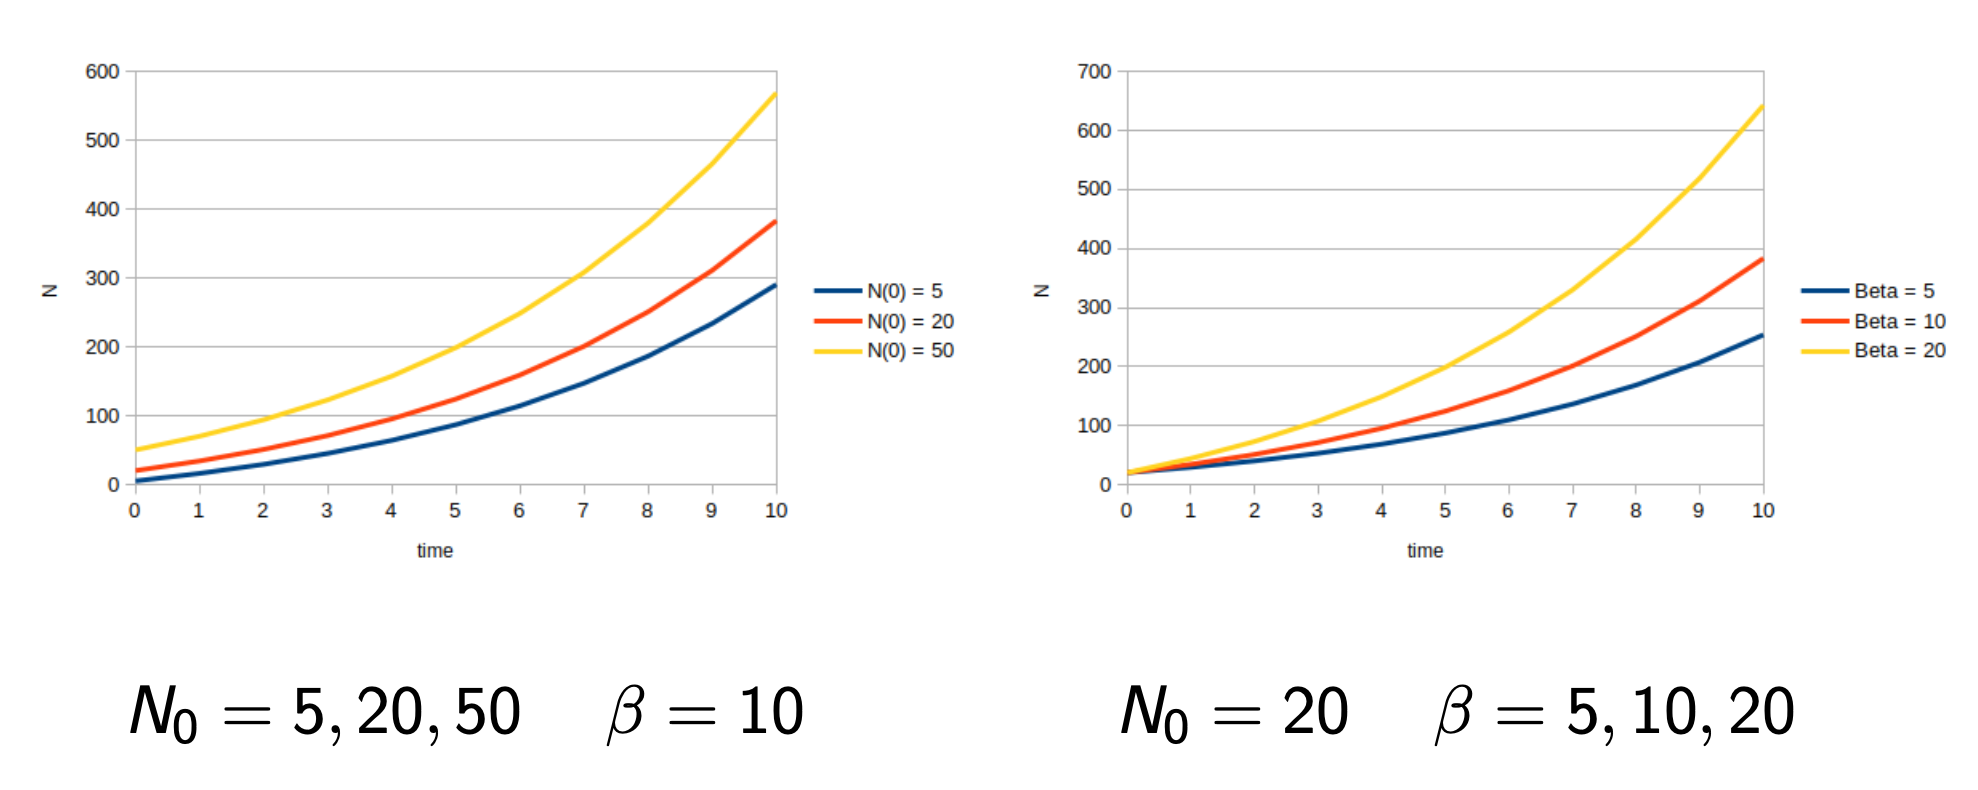
\includegraphics[width=0.9\textwidth]{Images/02-Discrete Dynamical Systems/case_1.png}
    \caption{The dynamics is dominated by the birth process (exponential growth).} 
\end{figure}

\par \textbf{Case $\alpha_{d} = 1$}

\begin{figure}[h]
    \centering
    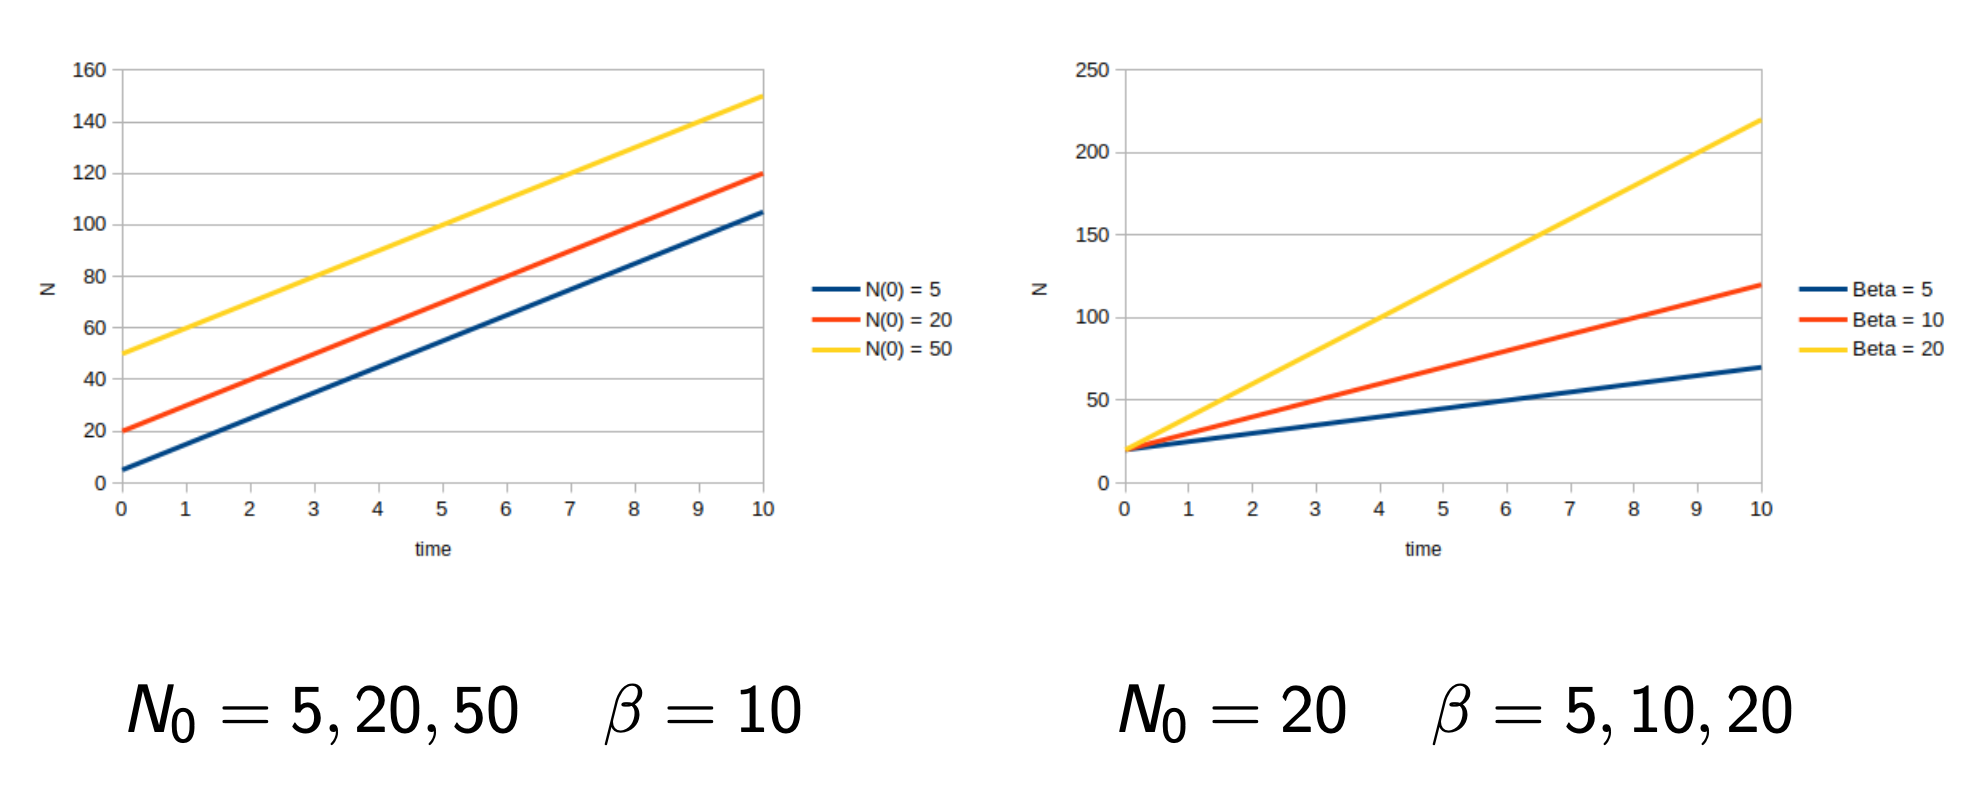
\includegraphics[width=0.9\textwidth]{Images/02-Discrete Dynamical Systems/case_2.png}
    \caption{The dynamics is dominated by the migration process (linear growth).} 
\end{figure}

\par \textbf{Case $\alpha_{d} < 1$}

\begin{figure}[h]
    \centering
    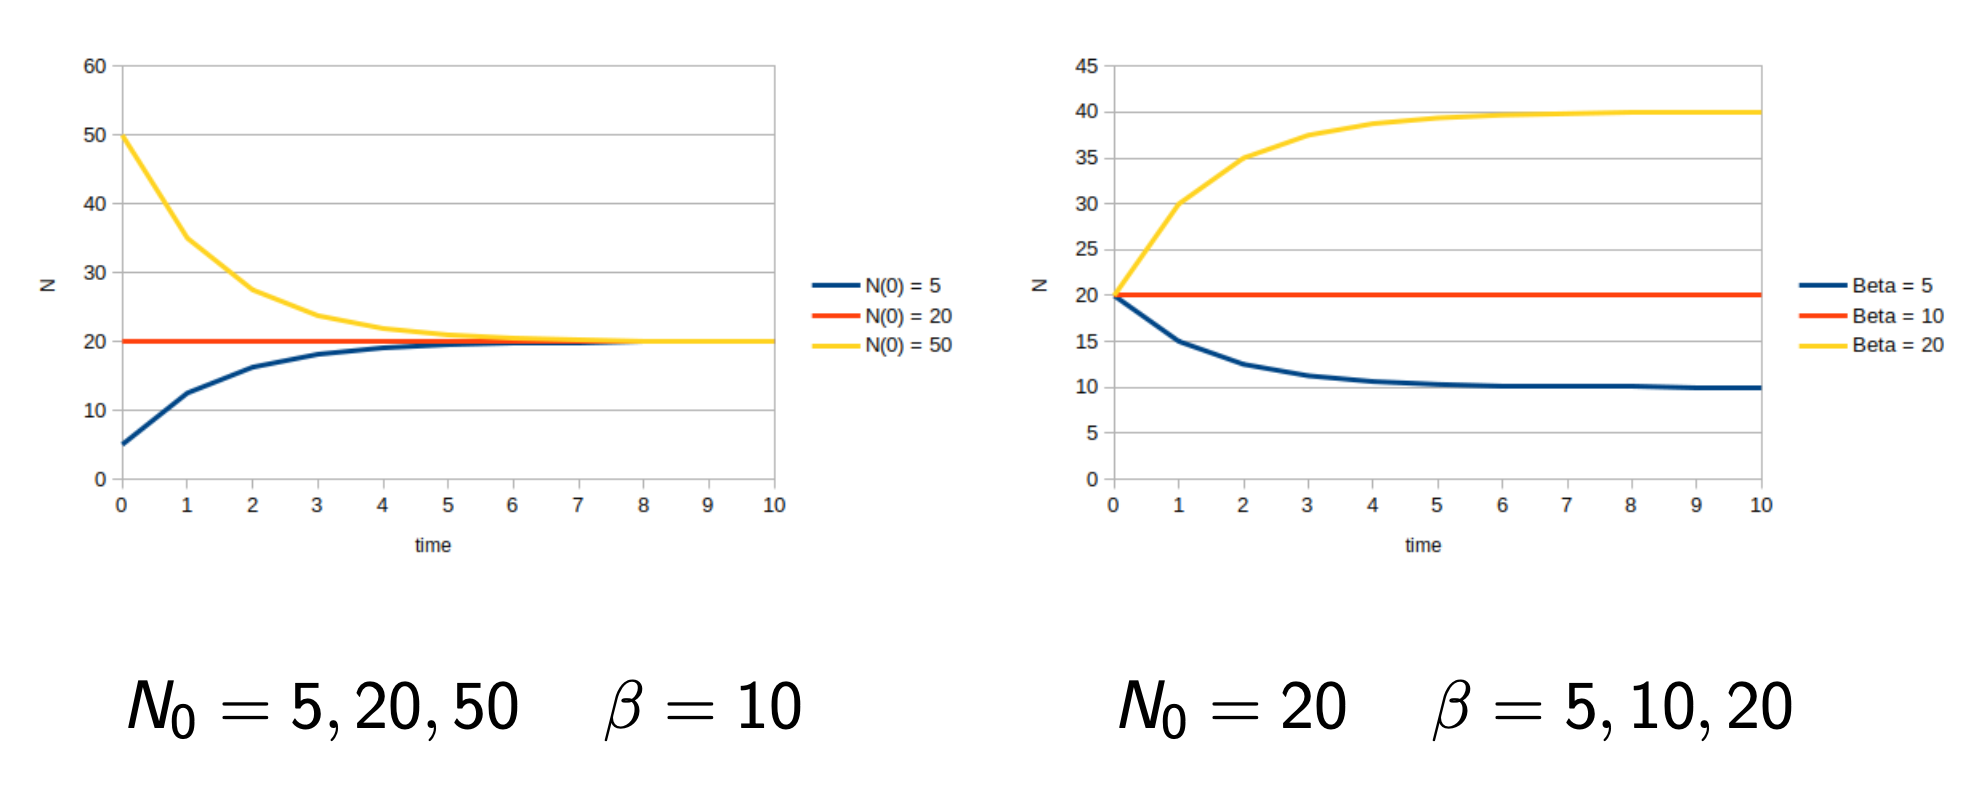
\includegraphics[width=0.9\textwidth]{Images/02-Discrete Dynamical Systems/case_3.png}
    \caption{The population reaches a dynamic equilibrium: a stable state in which opposite phenomena compensate each other (migration compensates deaths). Note that it is independent from $N_{0}$} 
\end{figure}

\subsection{Computing the equilibrium point}
The equilibrium point (also called saturation point) is defined as the moment $t=k+1$ where the computed size of the population is the same as the previous step, that is:

\begin{center}
    $N_{t-1} = N_{t}$
\end{center}

Knowing that $N_{t} = \alpha_{d}N_{t} + \beta$ we solve the equation in regards to $N_{t}$ and obtain:

\begin{center}
    $N_{t} = \frac{\beta}{1 - \alpha_{d}}$
\end{center}

\subsection{Non-linear models}
So far we have described a population where each individual behaves autonomously, which do not fit the definition of complex system (many components with very simple individual behaviour \textbf{that interact with each other and the environment}). Introducing interaction between the individuals \textbf{requires a non-linear model} (previously we used a linear one). In our (Non-linear) Birth Model now the environment has limited resources such as food and place, thus requiring that the individuals compete \textbf{(a form in interaction)} for survival.

\section{Rewriting our equation}
For simplicity assume we are in a closed environment (no migration), then we define $K$ as the \textbf{carrying capacity of the environment}, meaning that in the environment there is enough food and space for $K$ individuals.
\par The population is still governed by the birth rate, but now death is no more a constant, instead is negatively influenced by $K$:

\begin{center}
    $N_{t+1} = r_{d}N_{t}(1 - \frac{N_{t}}{K})$
\end{center}
\textbf{Note:} this non-linear equation is called \textbf{logistic equation} (it is an alternative formulation)

So now the birth rate is modulated by the ratio of occupancy on the environment $\frac{N_{t}}{K}$:

\begin{itemize}

    \item $N_{t}$ close to 0 : we have a simple birth process with rate $r_{d}$ (exponential growth). 

    \item $N_{t}$ increases: the growth tends to stop.

\end{itemize}

Eventually the population reaches a \textbf{dynamic equilibrium} representing the situation in which environment resources are fully exploited (\textbf{saturation})

\begin{figure}[h]
    \centering
    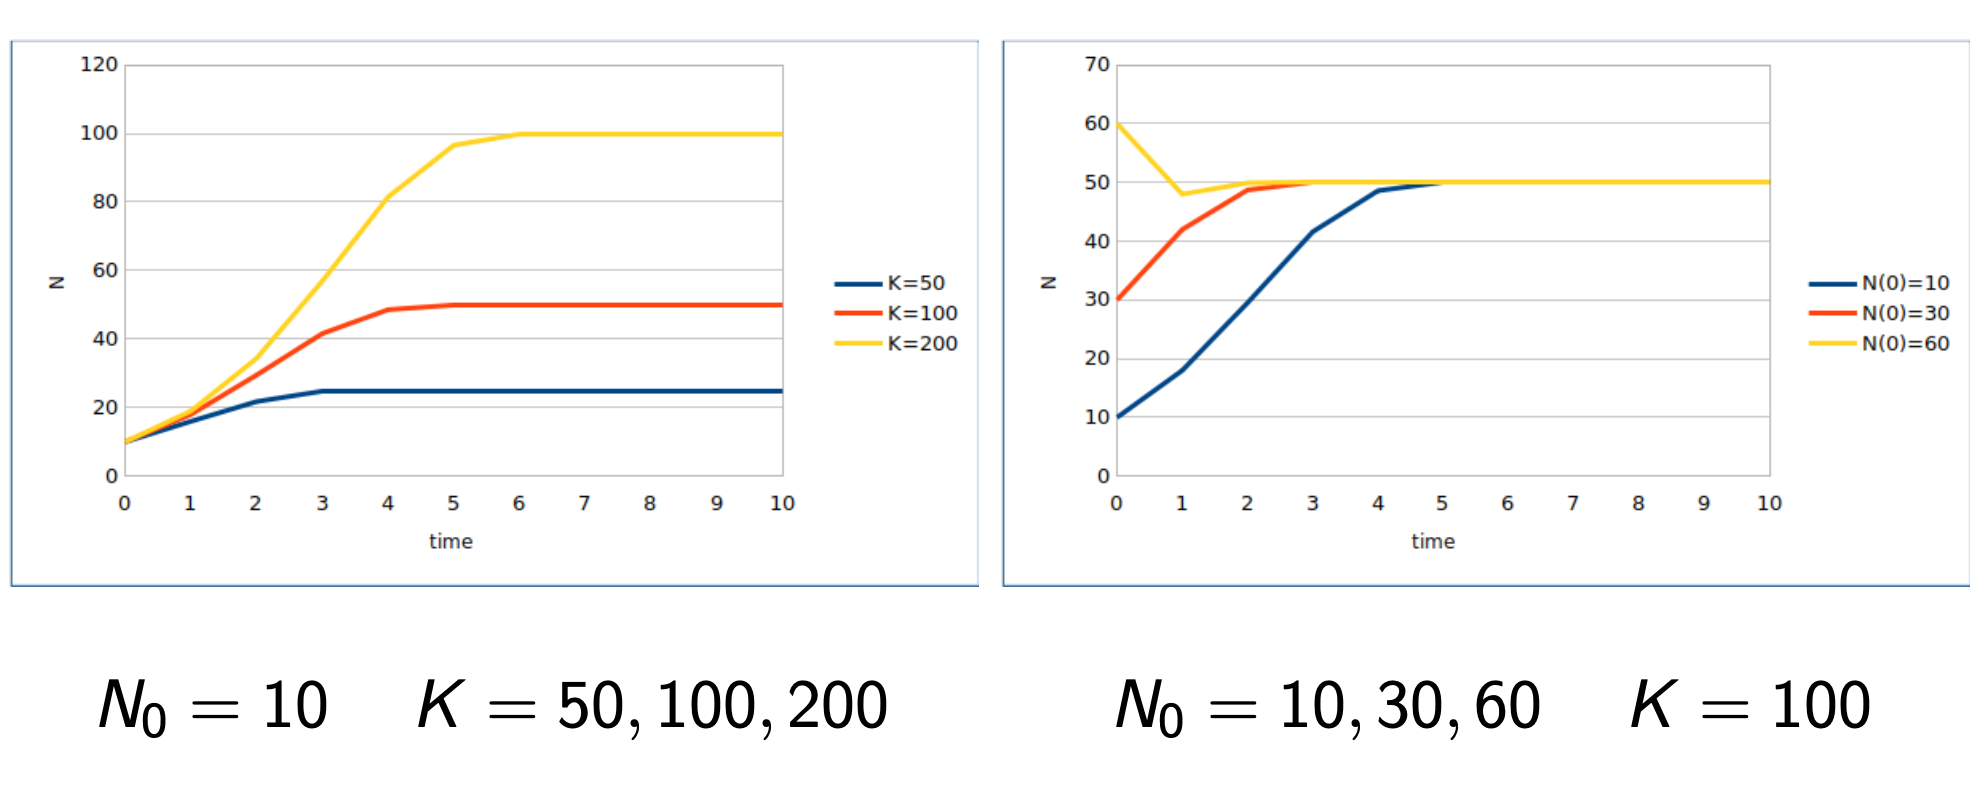
\includegraphics[width=0.9\textwidth]{Images/02-Discrete Dynamical Systems/Non-linear .png}
    \caption{The first graph shows a case where the equilibrium point depends on $K$. The second graph shows me that the equilibrium point is independent from the initial number of individuals.} 
\end{figure}

\section{Removing homogeneity}
For now we have considered an homogeneous population, but in realistic case we have different individuals with different features and we want to consider each group of individuals. In the system point of view this requires not just a single recurrence equation, but a \textbf{system of recurrence equations}. 
\par consider a population of fishes that live in a pond. Each individual can either be a male fish, modelled as $M_t$ or a female fish, modelled as $F_t$. We consider that a small part of males dies because of fights among them (death rate $s_d$).
\par then we construct a system of recurrence equations:


\[
\begin{cases}
    \begin{aligned}
        F_{t+1} = r_{d}F_{t}(1 - \frac{F_{t} + M_{t}} {K}) \\
        M_{t+1} = r_{d}F_{t}(1 - \frac{F_{t} + M_{t}}{K}) - s_{d}M_{t}\\
    \end{aligned}
\end{cases}
\]

where:
\begin{itemize}
    \item $r_{d}F_{t}$ represent the number of child born, note that they are generated by females.

    \item $F_{t} + M_{t}$ describes the whole population size (to be related with the carrying capacity K).
\end{itemize}

\section{Limitation of discrete dynamical models}
Discretization of the system dynamics may introduce inaccuracies: recurrence equations assume that nothing happens during the $\Delta{t}$ time that occurs between $N_{t}$ and $N_{t+1}$. Adjusting $\Delta{t}$ to be smaller usually correspond to more accurate approximations, more precisely we should let $\Delta{t}$ tend to 0.


\chapter{Continuous Dynamical Systems}

\section {Recap - Why we need to introduce ODEs}
As we said in the previous chapter, using a discrete representation for the steps in our model can lead us to lose all the informations that happens between the step $N_t$ and the step $N_t+1$. \par
The simplest solution is to make the distance in time $\Delta t$ between the to step very small ($\approx 0$), but it is not enough.

\section{Reconsidering the population model}
Recall in our population model that with $N(t)$ we denote the \textbf{density of some population} at time t. Our goal is to construct a mathematical model able to predict the density of the same population at a time $t^{'} = t + \Delta{t}$.

\subsection {Introducing the Ordinary Differential Equation}

\par Given our equation which is based the model:
\begin{center}
    $N(t + \Delta{t}) = N(t) + \lambda{\frac{\Delta{t}}{\sigma}{N(t)}}$
\end{center}
And the corresponding \textbf{recurrence equation}:
\begin{center}
    $N_{t+1} = r_{d}N_{t}$
\end{center}
where $r_{d} = \frac{\Delta{t}}{\sigma}$ consider the case where $\Delta{t} \rightarrow 0$. This case cannot be done using discretization, because it can lead to inaccuracies.
\par To handle the case $\Delta{t} \rightarrow 0$ we make some transformation to our equation:

\begin{center}
    $N(t + \Delta{t}) = N(t) + \lambda{\frac{\Delta{t}}{\sigma}{N(t)}} \rightarrow  \frac{N(t + \Delta{t}) - N(t)}{\Delta{t}} $
\end{center}

then by simplifying we get:

\begin{center}
    $ \frac{N(t + \Delta{t}) - N(t)}{\Delta{t}} = \frac{\lambda}{\sigma}N(t) $
\end{center}

We can recognize that the left hand side can be traced back as the \textbf{difference quotient} $\frac{f(x + h) - f(x)}{h}$, \textbf{which when taken to the limit as h approaches 0 gives the derivative of the function f}.
\par Let's consider our equation for $\Delta{t} \rightarrow 0$:

\begin{center}
    $\lim_{\Delta{t} \to 0} \frac{N(t + \Delta{t}) - N(t)}{\Delta{t}} 
    = 
    \lim_{\Delta{t} \to 0} r_{c}N(t)$
\end{center}

with $r_{c} = \frac{\lambda}{\sigma}$

Note that on the right hand side $\Delta{t}$ doesn't appear, thus we can remove the limit; the term on the left hand side is the derivative of $N(t)$, indicated as simply $\dot{N}(t)$. Thus we simply the equation as follows:

\begin{center}
    $\dot{N}(t) = r_{c}N(t)$
\end{center}

We have defined the dynamics of the system as the derivative equal to a constant multiplied by the value of the function at time $t$.\par \textbf{This equation is known as Ordinary Differential Equation (ODE)}.
\par An ODE has the following properties:
\begin{itemize}
    \item it relates the function $N$ with its derivative $\dot{N}$

    \item $t \in \mathbb{R}$, \textbf{so time is continuous}
\end{itemize}

\par We would like to use the Ordinary Differential Equation to run some simulation or to compute a general solution (like we did for the recurrence relation). 

\subsection{Using the ODE}
In some very simple case, like our linear birth model, we can find the general solution by finding a closed-form definition of $N(t)$ satisfying the equation. \textbf{A closed-form definition is one that depends only on t and some constant}. 
\par for the linear growth model a solution can be found analytically. 

\par Recall our equation:
\begin{center}
    $\dot{N}(t) = r_{c}N(t)$
\end{center}
Now let's move $N(t)$ from the right to the left hand-side of the equation:

\begin{center}
    $\frac{\dot{N}(t)}{N(t)} = r_{c}$
\end{center}
Recall that $\frac{\dot{N}(t)}{N(t)} = \ln{N(t)}$ and $r_{c}$ is the derivative of $r_{c}t + c$ for any constant $c$, obtaining:

\begin{center}
    $\ln{N(t)} = r_{c}t + c$
\end{center}
By resolving our equation in regards to $N(t)$ we finally get:
\begin{center}
    ${N(t)} = Ce^{r_{c}t + c}$
\end{center}
where $C = e^{c}$ (typically $C$ is set to be equal to $N(0)$

\begin{figure}[h]
    \centering
    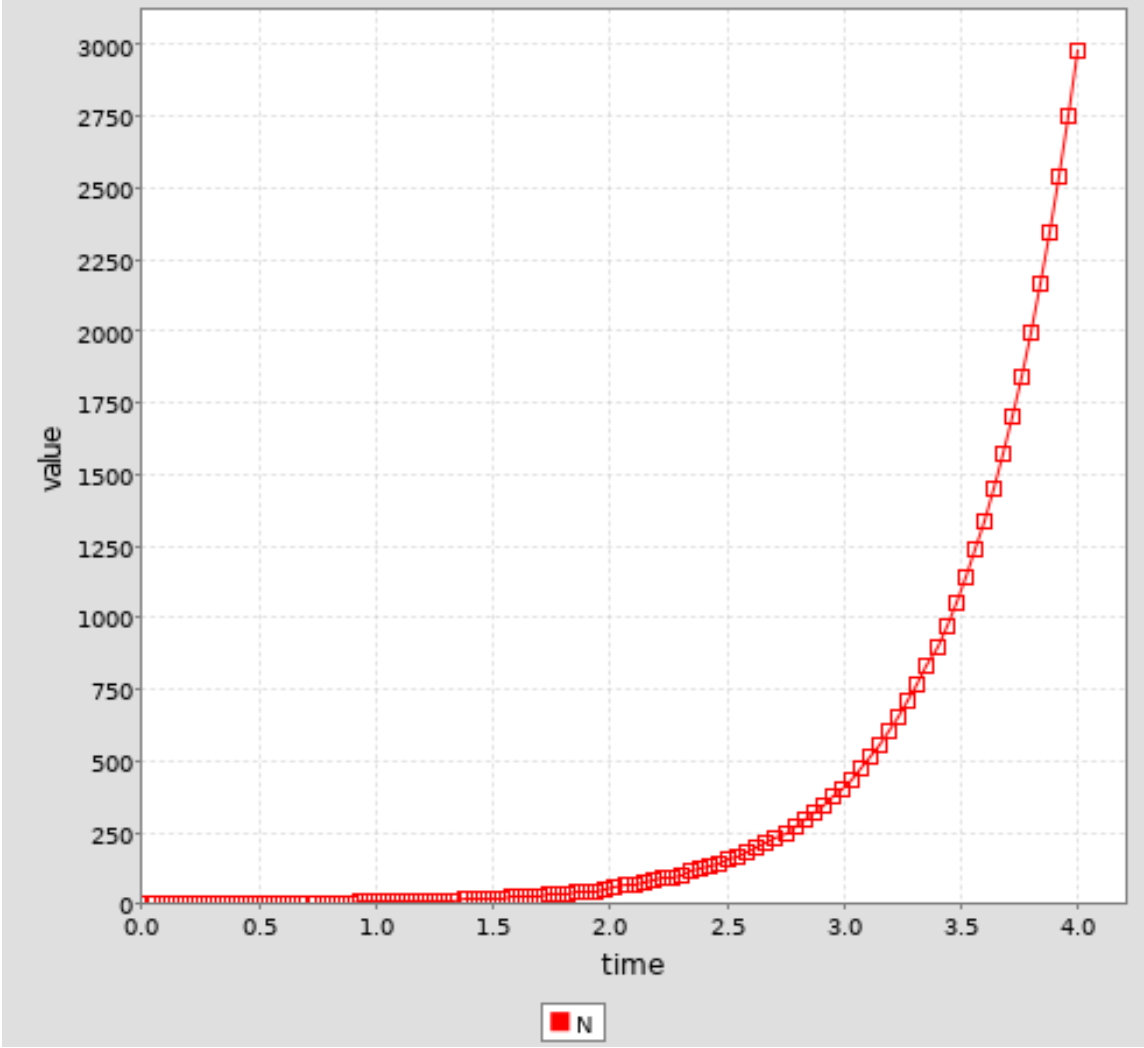
\includegraphics[width=0.5\textwidth]{Images/03 - Contiguous Dynamicsl System/linear_birth_model_continuous.png}
    \caption{This graphs shows us that by setting in our population model $r_{c} = 2$ and $C = N(0) = 1$ then the population shows an exponential growth over time.} 
\end{figure}

\subsubsection{Differences between discrete and continuous model}
This behaviour is qualitatively the same as for the discrete model, both showing exponential growth.
\textbf{What changes is the meaning of the equation}: 
\begin{itemize}
    \item the recurrence relation tells you how to update the variable.

    \item in our new equation it defines the derivative, \textbf{meaning how fast it's changing}.
\end{itemize}
Note how both equations show rate $\geq 1$ only if the birth rate $\frac{\lambda}{\sigma}$ is $\geq 1$.

\section{Example - Radioactive decay}
We move from the example of the population model we have seen so far to another one.
\par Radioactive decay is a process where we have a negative evolution of the population. The idea is that \textbf{each molecule decays at a constant rate}, so the whole mass decreases with a rate which is proportional to the mass itself.
\par We can describe this model by using the following Ordinary Differential Equation:

\begin{center}
    $\dot{N}(t) = -d_{c}N(t)$
\end{center}
then if we solve it in regards to $N(t)$ we get:
\begin{center}
    $N(t) = N(0)e^{-d_{c}t}$
\end{center}

\begin{figure}[h]
    \centering
    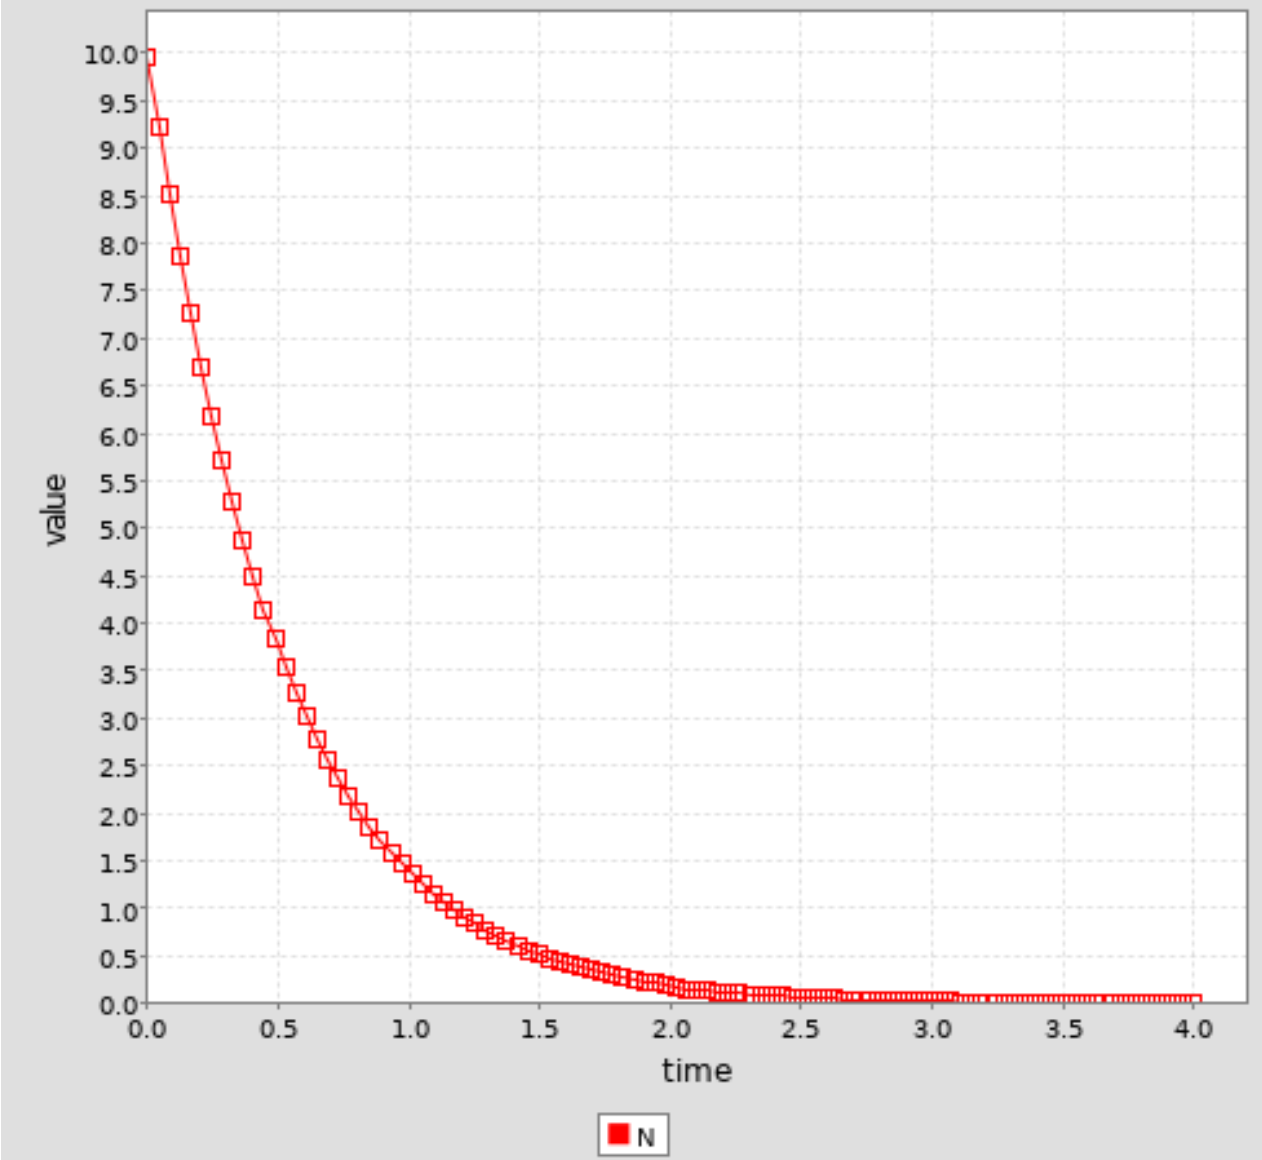
\includegraphics[width=0.5\textwidth]{Images/03 - Contiguous Dynamicsl System/Radioactive_decay.png}
    \caption{Example of applying the ODE of the radioactive decay. Note that  by setting $d_{c} = 2$ and $C = N(0) = 10$ we get $N(t)$ to tend to zero. This is caused by the negative exponent in the ODE.} 
\end{figure}

\section{Continuous version of the logistic equation}
Given the non-linear logistic equation, we can define as follows its continuous version:
\begin{center}
    $\dot{N}(t) = r_{c}N(t)(1 - \frac{N(t)}{K})$
\end{center}
where:
\begin{itemize}
    \item $r_{c}$ is the \textbf{continuous growth rate}.

    \item $K$ is the \textbf{carrying capacity} of the environment.
\end{itemize}

Resolving the ODE in regards to $N(t)$ we get:
\begin{center}
    $N(t) = \frac{K}{1 + (\frac{K}{N(0)} - 1) e^{-r_{c}t}}$
\end{center}
We notice that when $N(t) \rightarrow K$ \textbf{the population converges to the carrying capacity of the environment}.

\begin{figure}[h]
    \centering
    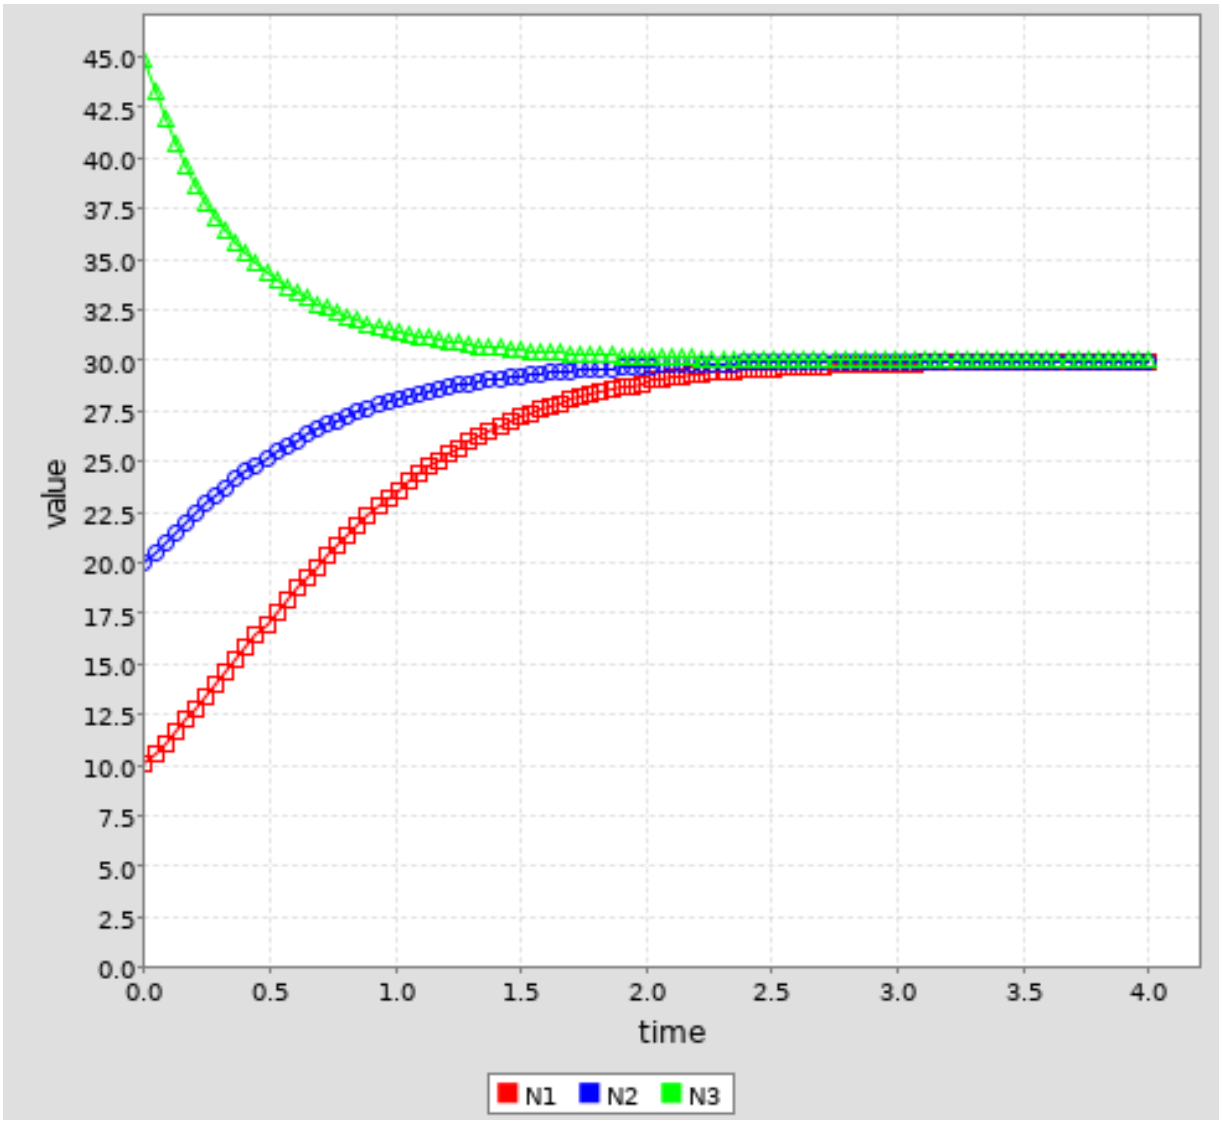
\includegraphics[width=0.5\textwidth]{Images/03 - Contiguous Dynamicsl System/continuous_logistics.png}
    \caption{Example of the continuous logistic equation. Note how by putting $r_{c} = 2$, $N(0) = 10$, $K = 30$, the population will eventually converge to the carrying capacity of the environment.} 
\end{figure}

\par \textbf{The trend is the same as for the discrete case}.

\section{Systems of ODE}
Now let's consider a population of males, indicated as $M(t)$, and females, indicated as $F(t)$. Assume that males fight with each other, so a small part of them dies because of it with a death rate of $s_{c}$. 
\par Thus we have to expand our model considering a system of ODEs:
\[
\begin{cases}
    \begin{aligned}
        \dot{F}_{t} = r_{c}F_{t}(1 - \frac{F_{t} + M_{t}} {K}) \\
        \dot{M}_{t} = r_{c}F_{t}(1 - \frac{F_{t} + M_{t}}{K}) - s_{c}M_{t}\\
    \end{aligned}
\end{cases}
\]
where:
\begin{itemize}
    \item $r_{c}F(t)$ is used for both genders, \textbf{since both are generated by females}.
    \item $F(t) + M(t)$ describes the whole population size.
\end{itemize}

\begin{figure}[h]
    \centering
    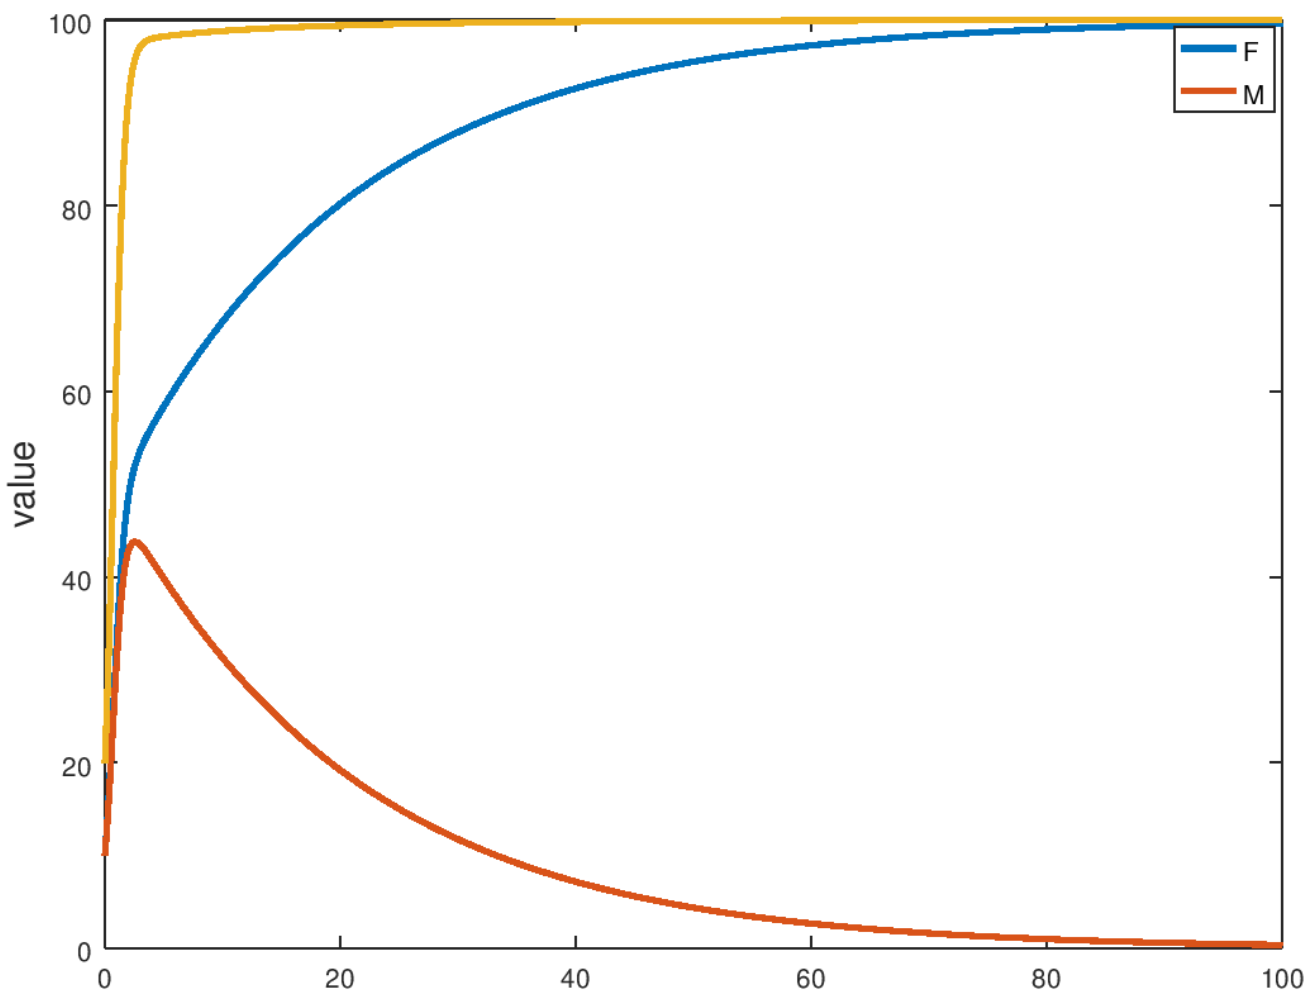
\includegraphics[width=0.5\textwidth]{Images/03 - Contiguous Dynamicsl System/system of ODE.png}
    \caption{Example of the system of ODEs.} 
\end{figure}

What happens in this scenario, after some times you have only females in the population. This shows a completely different behaviour from the discrete case, \textbf{because the meaning of their equations is different}:
\begin{itemize}
    \item The recurrence relations indicates us the size of the population.

    \item The system of ODEs describes how fast is changing.
\end{itemize}

\section{Numerical Solution of ODEs}
Recall that we said that computing the solution of an ODE is not always possible. For this reason we prefer working using an approximation of the solution, indicated as \textbf{numerical solver} (or numerical simulator). This approximation doesn't compute the general function, \textbf{instead it solves the initial value problem, also called Cauchy problem}.

\begin{center}
\subsubsection{Initial Value Problem}
Given an ODE in the form $\dot{N}(t) = f(N(t)) $ and an initial value $N_{0}$ s.t. $N(0) = N_{0}$, compute a function $F(t)$ that is a solution of the ODE and s.t. $F(0) = N_{0}$.
\end{center}

In our case we are interested only in studying the values of $F(t)$ where $t \geq 0$, \textbf{hence we perform a numerical simulation starting at} $t = 0$.

\section{The Euler method}
The Euler method is the simplest numerical simulation method available. The main concept behind this approach is to approximate the given continuous system with a recurrence relation specifically designed to approximate the continuous differential equation. \textbf{The idea is that, since we know the derivative, we use it as it was the function}.\par
It is based on the idea of discretizing the dynamics of differential equations by time steps of constant length $\tau = \Delta t$.\par
Given an Ordinary Differential Equation in the form:

\begin{center}
$\dot{N}(t) = f(N(t))$ 
\end{center}
this corresponds to approximating its solution with the following recurrence relation (assuming $N_0 = N(0)$) 
\begin{center}
$N_{k+1} = N_k + \tau f(N_k)$ 
\end{center}
where $N_k \approx N(\tau k)$

\begin{figure}[h]
    \centering
    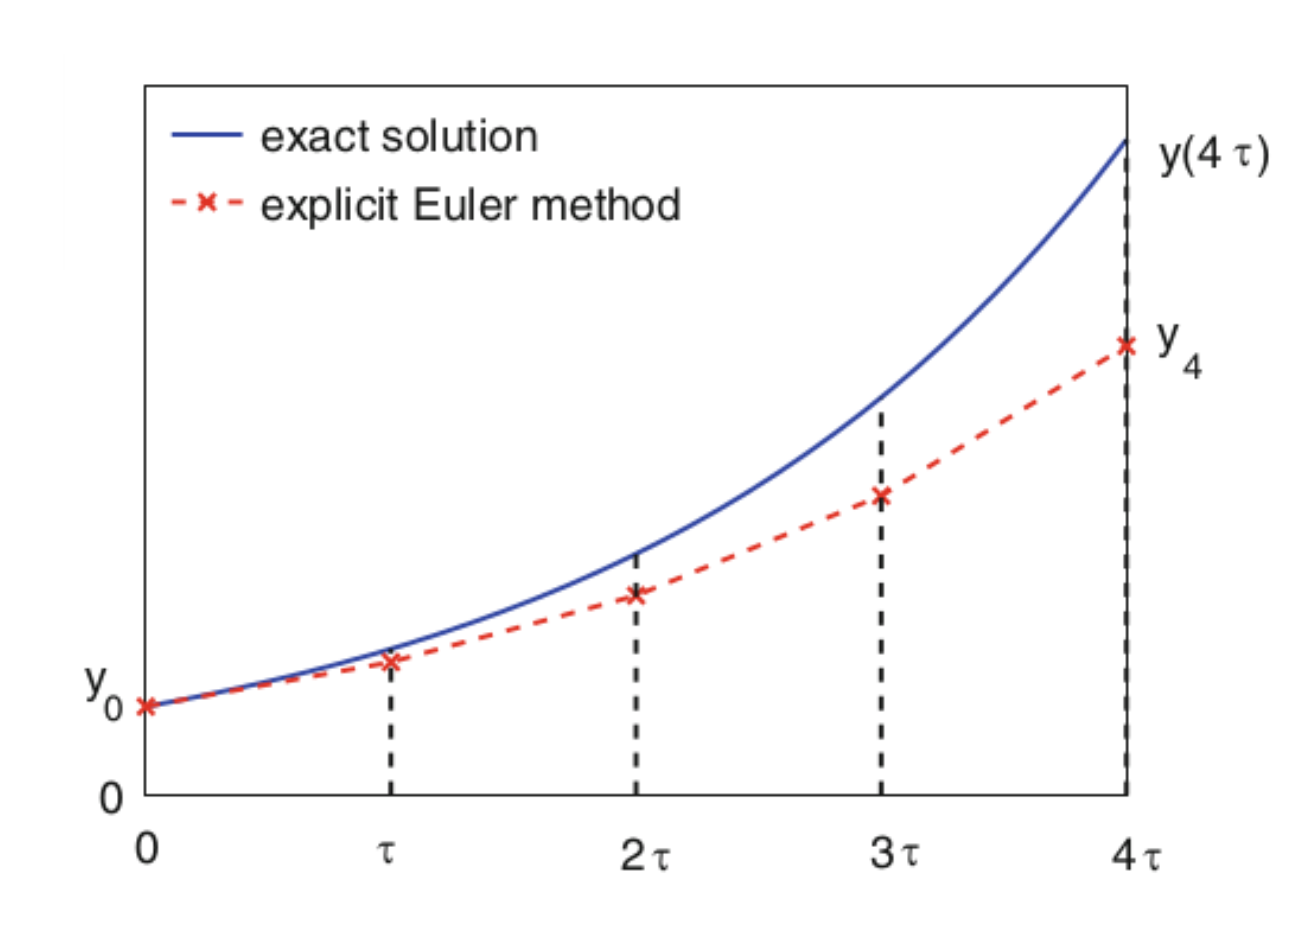
\includegraphics[width=0.5\textwidth]{Images/03 - Contiguous Dynamicsl System/Euler_method.png}
    \caption{A graph showing the correct solution compared to the approximation generated by the Euler method.} 
\end{figure}

\subsection{Errors in the Euler method}
By approximating in each step the Euler method makes local errors that will contribute to a global error at the end of the whole simulation.\par

\textbf{The local discretization error} is computed as $| N(\tau) - N_1|$ and it is in the order of $O(\tau^2)$ \textit{(the motivation is because we truncate the Taylor Series at the first step)}.\par

\textbf{The Global discretization error} is obtained by accumulate all the local discretization errors after $k$ steps, namely at time $t = k \tau$. The global error is computes as $|N(k \tau) - N_k)$ and is in the order $O(k \tau^2) = O(\tau)$ since $k \tau = t$ is constant.

\section {Other numerical simulation methods}
A linear error of $O(\tau))$ is quite annoying, requiring us to set $\tau \approx 0$ in order to have something acceptable, making the computation very slow (it requires a lot of steps).\par
To overcome this other methods have been proposed, having a global discretization error of a higher order (e.g. $O(\tau^p)$ for some p) which is better as long as $\tau \rightarrow 0$ (hence $\tau < 1$). To work these method use more than one point to approximate the value of the function, making a single step require more time, but maintain the error inside some defined boundaries. \par

A few examples of such methods are:
\begin{itemize}
    \item \textbf{Runge-Kutta methods:} $p = 2$ in the original formulation, but can be higher
    \item \textbf{Multistep methods (e.g. Adams methods):} extrapolate the value of the next step from the values of the previous k steps obtaining $p \approx k$.
\end{itemize}

State-of-art methods can also:
\begin{itemize}
    \item \textbf self-determine the step size $\tau$ based on thresholds on local and global discretization errors.
    \item \textbf dynamically adjust the step size $\tau$ during their executing (e.g. Adaptive Runge-Kutta) 
\end{itemize}

\section{Instability and stiff systems}
There is another problem that could arise: if you have a derivative which cause the value of a variable in a very fast way, if $\tau$ is not small enough you not only pay some error but you could have that your computed solution is unstable.\par
What we mean for unstable is that we lose informations and your points start to oscillate creating chaos.\par

\begin{figure}[h]
    \centering
    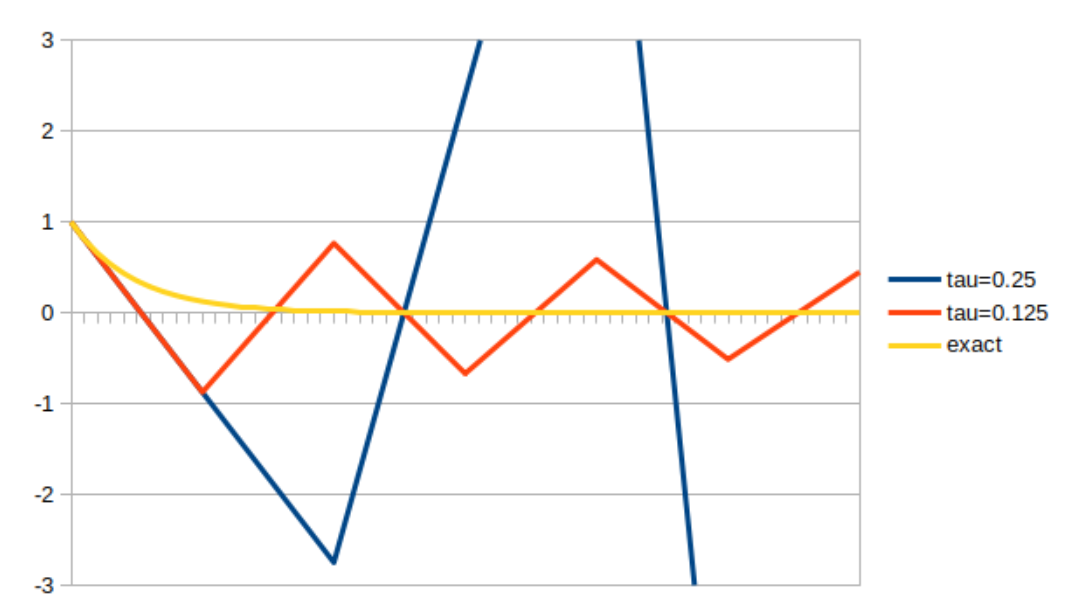
\includegraphics[width=0.5\textwidth]{Images/03 - Contiguous Dynamicsl System/Stiff System.png}
    \caption{An example of a stiff system. In orange is shown the real solution, while in red and blue the one obtained by setting $\tau$ to different values} 
\end{figure}

This kind of problematic systems are called \textbf{stiff systems}. There is no clear definition of stiffness: intuitively contains a very fast term that cannot be captured by our method, worse if we have in our systems also slow terms to take into account. \par
In this cases you need to consider alternative numerical simulation methods called \textbf{implicit numerical simulation methods}. All the methods we have seen so far have and implicit version, which requires more computation time for step.

\section{Implicit Euler method}
The idea of the implicit version of the Euler method is that, like the previous version we approximate the function by using its derivative, \textbf{but the derivative is not computed on the value $N$ at step $k$, but at the step $k+1$}.\par
By using this approach we are no longer defining $N_{k+1}$ in terms of $N_k$, but as an equation where $N_{k+1}$ is in both sides:

\begin{center}
    $N_{k+1} = N_{k} + \tau f (N_{k+1})$
\end{center}
where $N_k \approx N(k \tau)$.\par

There are methods from numerical analysis that are able to solve these type of equations. This method requires more effort for computing a single step, but \textbf{often} the local discretization error is smaller permitting us to use greater values of $\tau$.

\section{Other implicit methods}
Implementations of implicit methods that use more than one variables require the modeler to provide the \textbf{Jacobian matrix} (partial derivatives) of the function f. Most are able to compute the Jacobian matrix autonomously by doing some approximation. \par
There exist methods that are able to automatically switch from explicit to implicit methods by determining if the system is stiff.





\chapter{Relevant Examples of ODEs}

\section{Changing the notation}
In the ODEs that follows we will omit any explicit reference to the time variable t:

\begin{itemize}
    \item $X(t)$ will be just called $X$
    \item $\dot{X(t)}$ will be just called $X$
    \item $X_0$ will be just called $X(0)$
\end{itemize}

\section{The Lotka-Volterra model of prey-predator interaction}
These are two independent model that resulted to be equivalent:
\begin{itemize}
    \item \textit{Lotka} designed in 1925 as a description of an hypothetical biochemical oscillator.
    \item \textit{Volterra} designed in 1926 as a description of two interacting populations.
\end{itemize}

\subsection{Introduction}
Volterra's model was made to explain a strange phenomenon observed in the Adriatic sea after World War 1. During the war there was a increasing demand of fish, so ecologist and fisherman predicted that the overall population of fish would decrease. To everyone surprise after the Wold War ended, they observed an increase in population for some species.\par
Volterra's idea was that prey and predator have different \textbf{(but related)} dynamics. \textbf{The main intuition was that preys proliferate in the absence of predators}.\par

\subsection{Making the model}
First we abstract the prey population and predator population in the following variables that uses absolute numbers:

\begin{itemize}
    \item \textbf{V:} describes the size (also called density) of the population of preys.
    \item \textbf{B:} describes the size (also called density) of the population of predators.
\end{itemize}

We the make some basic observation regarding the inner dynamics of preys and predators \textbf{when they are isolated from each other}:

\begin{itemize}
    \item When there are no predators, preys can grow without any limitation.
    \item When there are no preys, predators die of starvation.
\end{itemize}

We design a preliminary system of ODEs for describing these observations:

\begin{itemize}
    \item $\dot{V} = rV$ where $r$ is the \textbf{growth rate of preys}.
    \item $\dot{P} = - sP$ where $s$ is the \textbf{death rate of predators}.
\end{itemize}

\subsubsection{Digression}
When you construct a model you can follow two approaches:
\begin{itemize}
    \item Try to model all the possible details in the most accurate way you can. This will lead you to a very complicated model, but if you are able to take all the aspect of the system into account by measuring correctly the parameters introduced, then you should be able to replicate the reality. \textbf{So you can make quantitively prediction about that model.} However this can make the analysis difficult because if you want to explain a certain dynamics, it may be hidden behind all the parameters you have.

    \item Try having a minimal model when you put only the details you think are necessary to understand the trend you want to predict. Then although quantitive prediction are wrong, you will have a more clear observation of the trend.
\end{itemize}

\textbf{Volterra's model follow the second approach.}

\subsection{Interaction between the two species}
We have developed a system of ODEs in the case when the two species are separated from each other, but what about when both species are present in the environment? \textbf{We observe that the predators hunts the preys}. How can I model hunting in a minimal way? \par
Assuming that a prey and a predator meet, then the predator eats the pray and increases the change of growth of is population. Assuming that the meeting between individuals of both species is random, then to model it we add one term in each of the ODEs in our system:

\begin{itemize}
    \item In the predator ODE it has a positive sign because by eating the pray it increases the chance of survival of its population
    \item in the predator ODE it has a negative sign because by being eaten it decreases the chance of survival of its population
\end{itemize}


The first intuition was that predation is proportional to the quantity of pray and predators. The rate of predations should be proportional to the quantity of meetings between individuals of the two species \textbf{(namely it is proportional to the product $V * P$)}. Note that the \textbf{meeting between individuals is random}.\par
When a prey and a predator meet, it could happen that the predator eats the prey, \textbf{but not always}. 
\begin{itemize}
    \item So we declare $a$ as the portion of meetings resulting in huntings (the predator eats the prey).
\end{itemize}

As the predators eat, their chance of survival increases and they start to reproduce. 
\begin{itemize}
    \item So we declare $b$ as the number of offsprings produced for each huntings.
\end{itemize}

\subsection{Putting all together}
By inserting in our system of ODEs the considerations we have made we obtain:

\[
\begin{cases}
        \dot{V} = rV - aVP \\
        \dot{P} = - sP + abVP\\
\end{cases}
\]

\begin{itemize}
    \item \textbf{First ODE:} it tells us that prey decrease by the \textbf{hunting rate} $aVP$.
    \item \textbf{Second ODE:} it tells us that predators increase by a \textbf{hunting and reproduction rate} $abVP$.
\end{itemize}

We have modelled predation as a direct form of interaction, \textbf{it is not mediated by the environment}

\section{Steady State}
A steady state is a combination of values for the variables that remains unchanged over time. \textbf{In a steady state, all differential equations are equal to zero}.

\section{Example - The SIR epidemic models}
Epidemic phenomena deals with the spread of infectuous diseases. To study them there are used SIR models. 

\subsection{Introduction}
SIR stands for the three types of individuals in our population:

\begin{itemize}
    \item \textbf{Susceptible:} individuals that can be infected.
    \item \textbf{Infected:} infected individuals that can spread the disease to susceptible individuals.
    \item \textbf{Recovered:} infected individuals who passed the infection phase and cannot spread the disease anymore.
\end{itemize}

There are several variants of the SIR model, some being developed during the COVID pandemic.

\subsection{Making the model}
We design a Ordinary Differential Equation for each type of individual in our population, each ODE describes the ratios of each class of individual:

\begin{itemize}
    \item \textbf{S:} ODE for the Susceptible type.
    \item \textbf{I:} ODE for the Infected type.
    \item \textbf{R:} ODE for the Recovered type.
\end{itemize}

We make the following assumption:

\begin{itemize}
    \item The size of the population is constant in time and normalized to 1: $S + I + R = 1$.
    \item Infected people can only transmit the infection, meaning they \textbf{cannot} reproduce, die, migrate and so on.
    \item A infected person can transmit the disease only to susceptible people through personal contact between the two (horizontal transmission).
    \item The contact between individuals is random, meaning the number of infections is proportional to both I and S.
    \item After being Infected a person will recover become resistant to that disease.
\end{itemize}

Following these assumption we can represent the model as the following system of equations:

\[
\begin{cases}
        \dot{S} = - \beta S I \\
        \dot{I} = \beta S I - \gamma I\\
        \dot{R} = \gamma I \\
\end{cases}
\]

where:

\begin{itemize}
    \item $\beta$: is the \textbf{infection coefficient} describing probability of infection after the contact between a susceptible individual and an infected one.
    \item $\gamma$: is the \textbf{recovery coefficient} describing the rate of recovery of each infected individual.
\end{itemize}

\subsubsection{Dynamic between S and R}
S and are have a very intuitive dynamic: S having only a negative sign will inevitably decrease, while R having only a positive sign will increase. \par

In the case of I, its behaviour strictly depends on the value of $\beta$ and $\gamma$, more precisely:

\begin{itemize}
    \item if $\beta < \gamma$: then I will decrease (since S $\leq$ 1)
    \item if $\beta > \gamma$: then the behaviour of I depends on S. If $S > \frac{\gamma}{\beta}$ then I will increase its value.
\end{itemize}

\subsection{Extending the model - Vaccination}
The SIR model can be used to study the effects of vaccinations: considering if its convenient or not to introduce mandatory vaccination for some diseases. \par
To better study vaccinations you need to consider the model for several years. For instance if you vaccinates newborns, you will see the result of your choice only after they will become the main part of your population. By considering a long time span \textbf{births and deaths cannot be ignored}, so we need to extend our SIR model.

\par idea: we add a positive terms to represents births and add a negative terms to represent death. To make this work we will use the following assumptions:

\begin{itemize}
    \item \textbf{the population size is still constant over time} (not too wrong: the size of the population of a country does not change significantly over 10-20 years).
    \item No vertical transmission of the disease (meaning from parent to children.
    \item Newborns are considered Susceptible from the get go.
\end{itemize}

To make the population constant we introduce the coefficient $\mu$ for both birth and death. Consider that the population size is normalized to 1. We declare with $N$ the population size s.t. $N = S + I + R$ and $\dot{N} = \mu - \mu N$.

Made these assumption we can extend the model obtaining the following system of ODEs:

\[
\begin{cases}
        \dot{S} = \mu - \beta S I \\
        \dot{I} = \beta S I - \gamma I\\
        \dot{R} = \gamma I\\
\end{cases}
\]

\textbf{Remember:} we are assuming that all type of people could reproduce, but the newborns are always Susceptible, since we are not considering vertical transmission. Thus in the ODE of S we put $]\mu$ alone to represent the number of people born during the current time unit.

\subsection{Introducing death}
As we have stated multiple times, the population size is assumed to be constant and normalized to 1. So having newborns in our model could lead us to an increase of the population, which is wrong. The solution is to introduce death in order to maintain the size. \par
The death is introduced by using the same parameter as the birth $\mu$, only with a negative sign. The obtained model will be:

\[
\begin{cases}
        \dot{S} = \mu - \beta S I - \mu S \\
        \dot{I} = \beta S I - \gamma I - \mu I\\
        \dot{R} = \gamma I - \mu R\\
\end{cases}
\]

The dynamics of the model is governed by the ration between the positive and negative coefficients in the equation of I:

\begin{itemize}
    \item $\beta < (\mu + \gamma)$: I can only decrease (since $S \leq 1$.
    \item $\beta > (\mu + \gamma)$: the behaviour of I depends on S. It increases if $S > \frac{(\mu + \gamma)}{\beta}$.
\end{itemize}

Note how compared to the previous case where S could only decrease, \textbf{now this is no longer true because the births could maintain S above} $\frac{\mu + \gamma}{\beta}$.

\subsection{Introducing vaccination}
Now let's consider the case where we can fight the disease by using vaccination.\par
We consider to vaccinates the newborns, the model can tell us if this will helps us and the fraction of newborns $p$ are needed to be vaccinated to do so. \par
We consider that if a newborn is vaccinated, then it has type Recovered.\par
The model we get is the following:

\[
\begin{cases}
        \dot{S} = (1-p)\mu - \beta S I - \mu S \\
        \dot{I} = \beta S I - \gamma I - \mu I\\
        \dot{R} = p \gamma I - \mu R\\
\end{cases}
\]

\subsection{Determining the vaccination threshold}
We declare with $p_c$ the thresgold value of vaccinations needed, that it the ratio of newborns that should be vaccinated in order to eradicate the disease.\par
There are two ways to compute $p_c$:

\begin{itemize}
    \item The value can be determined by simply performing numerical simulation varying the value of $p$

    \item The value of $p_c$ can be computed analytically.
\end{itemize}

By considering the second opition we obtain the following formula to compute the ratio:
 \begin{center}
     $p_c = 1 - \frac{\mu + \gamma}{\beta}$ 
 \end{center}

\section{Limitation of continuous dynamical models}
The main limitation of this approach is that they are deterministic: once you define the ODE and you fix an initial value for the variables you obtain \textbf{THE} only possible dynamics of the system. \par
In many cases there are aspects you did not model and there are events that can happen with some probabilistic distribution that you have not modelled here. To overcome this limitation we need to use a different modelling technique that introduce probability distribution in our model.

 
\chapter{The Chemical Reaction Metaphor}

Chemical reactions are illustrative examples of complex systems, they exhibit complex dynamics out of very simple interactions. 
Also chemical reaction are much easier to write than ODEs, so we will use them as a modelling language. \textbf{Chemical Reaction are used as a metaphor to describing interactions.}

\section{What is a chemical reaction?}
A chemical reaction is an interaction between molecules in a chemical solution that cause a transformation of these molecules. We categorize as:

\begin{itemize}
    \item \textbf{reactants:} the group of molecules that participate in the reaction.
    \item \textbf{products:} the group of molecules (it could be a different quantities that the reactants) that are obtained after the transformation.
\end{itemize}

We abstract molecules as symbols, \textbf{it does not matter what they are in the reality}. Molecules are assumed to be in a \textbf{chemical solution}, that is a fluid medium where they float. While in these solution they can meet and start a chemical reaction.\par
In order to represent the quantity of molecules is usually expressed in terms of \textbf{concentrations} (number of molecules per unit). \par
Given the molecule A, [A] denotes the concentration of that molecule, usually expressed in $\frac{mol}{L}$. \par

Usually the notation for chemical reactions is some sort of rule between the reactants and the products:

\begin{center}
    $\ell_1 S_1 + ... + \ell_p S_p \xrightarrow{k} \ell^{'}_1 P_1 + ... + \ell^{'}_\gamma P_\gamma$
\end{center}
where:
\begin{itemize}
    \item $S_i$ are \textbf{reactants}.
    \item $P_i$ are \textbf{products}.
    \item $\ell_{1}$, $\ell^{'}_{i} \in \mathbb{N}.$ are \textbf{stoichiometric coefficients}. They express the number of reactants/products of each type that are consumed/produced in the reaction
    \item $k \in \mathbb{N}_{\geq 0}$ is the \textbf{kinetic constant}. It express the rate of occurrence of reaction in a chemical solution.
\end{itemize}

Note: when we omit the $l_i$, it means that is value is $1$.

\subsection{Types of Chemical Reactions}

There are several types of chemical reactions:

\begin{itemize}
    \item \textbf{Synthesis:} $\xrightarrow{k} P$
    \item \textbf{Degradation:} $S \xrightarrow{k}$
    \item \textbf{Transformation:} $S \xrightarrow{k} P$
    \item \textbf{Binding:} $S_1 + S_2 \xrightarrow{k} P$
    \item \textbf{Unbinding:} $S \xrightarrow{k} P$
    \item \textbf{Catalysis:} $E + S \xrightarrow{k} E + P$
\end{itemize}
and many more

\subsubsection{Complex types as aggregation of simpler type}
Complex chemical reaction can be redefined as a sequence of simpler chemical reactions. Take for example the Catalysis ($E + S \xrightarrow{k} E + P$), it can be reinterpreted as a sequence of:

\begin{itemize}
    \item Binding: $E + S \xrightarrow{k} M$
    \item Transformation: $M \xrightarrow{k} N$
    \item Unbinding: $N \xrightarrow{k} E + P$
\end{itemize}

\subsection{Reversibility of Chemical Reactions}
Often chemical reactions can occur in both directions. To indicate formulas that are reversible we will use the symbol $\leftrightarrows^{k}_{k-1}$:

\begin{center}
    $\ell_1 S_1 + ... + \ell_p S_p \leftrightarrows^{k}_{k-1} \ell^{'}_1 P_1 + ... + \ell^{'}_\gamma P_\gamma$
\end{center}

where $k-1 in R_{\leq 0}$ is the kinetic constant of the inverse reaction, transforming products $P_i$ into reactants $S_i$.
\par In reality all chemical reaction are reversible, only one of the two direction is so unlikely that is not considered possible.

\subsection{The mass action kinetics of chemical reactions}
The dynamics of chemical reactions is based on the assumption that \textbf{molecules float in a well-stirred fluid medium} (e.g. water). In this scenario they are free to move and randomly meet each other. When two molecules meet, they can react.\par
The dynamics of chemical solution is modeled by the \textbf{law of mass action}

\subsubsection{Law of mass action}
The \textbf{rate} of a chemical reaction expresses the number of occurences of such a reaction in a given chemical solution in a time unit.\par
The law of \textbf{mass action} is an empirical law for the computation of the rate of chemical reaction:.\par

\begin{center}
    The rate of a chemical reaction is proportional to the product of the concentrations of its reactants.
\end{center}

Given the following chemical reaction:
\begin{center}
    $\ell_1 S_1 + ... + \ell_p S_p \xrightarrow{k} \ell^{'}_1 P_1 + ... + \ell^{'}_\gamma P_\gamma$
\end{center}

Then the rate of a reaction is defined as follows:
\begin{center}
    $k[S_{1}]^{\ell_{1}} ... [S_{p}]^{\ell_{p}}$
\end{center}

The rate of its inverse reaction (from right-to-left) is:
\begin{center}
    $k_{-1}[P_{1}]^{\ell^{'}_{1}} ... [P_{\gamma}]^{\ell^{'}_{\gamma}}$
\end{center}

\subsection{Understanding the kinetic constant}
What is the measure unit of a kinetic constant k?
It depends on the number of reactants:

\begin{itemize}
    \item The measure unit of \textbf{concentrations} is $\frac{mol}{L}$
    \item The measure unit of the \textbf{reaction rate} is $\frac{mol}{(L \times sec)}$ (it is the concentration of each product produced in one unit of time.
\end{itemize}
Note: some kinetic constants have to be changed if you change the measure unit of concentrations (e.g. $\mu mol$) or the time unit (e.g. hours).

\subsection{Dynamic equilibrium}
Given an initial concentration we can have an idea about which is the faster reaction that will take place among the one we have. Something we can compute is an equilibrium point for our reversible reactions. \par
Given a generic reversible reaction:
\begin{center}
    $\ell_1 S_1 + ... + \ell_p S_p \leftrightarrows^{k}_{k_{-1}} \ell^{'}_1 P_1 + ... + \ell^{'}_\gamma P_\gamma$
\end{center}
A dynamic equilibrium is \textbf{reached when the two rates are equal}:
\begin{center}
    $k[S_{1}]^{\ell_{1}} ... [S_{p}]^{\ell_{p}}$ $=$ $k_{-1}[P_{1}]^{\ell^{'}_{1}} ... [P_{\gamma}]^{\ell^{'}_{\gamma}}$
\end{center}

Then it is easy to compute the equilibrium using the following formula:
\begin{center}
    $\frac{k}{k_{-1}} = \frac{[P_{1}]^{\ell^{'}_{1}} ... [P_{\gamma}]^{\ell^{'}_{\gamma}}}{[S_{1}]^{\ell_{1}} ... [S_{p}]^{\ell_{p}}}$
\end{center}

\section{From chemical reactions to Ordinary Differential Equations}
We can use reaction rates to be able not only to compute point-wise rates and equilibrium point, but \textbf{to be able to analyse the dynamics of a system any time}.\par
Since rates are frequencies, \textbf{so some sort of derivative}, we can use them to define ODEs.\par
We will consider every molecule of the reaction as a variable of o our system of differential equation. Each molecule will have its own differential equation and then in each of these equations we will add positive and negative terms according to the reaction in which these molecules participates:

\begin{itemize}
    \item for every reaction where the molecule we are considering is a reactant, that is \textbf{it will be consumed to generate a product}, then its ODE will contain a negative term: $- \ell r$

    \item for every reaction where the molecule we are considering is a product, that is \textbf{it will be produced}, then its ODE will contain a positive term: $+ \elle r$
\end{itemize}

where:
\begin{itemize}
    \item $\elle$: is a \textbf{stoichiometric coefficient} of a product S in R.
    \item $r$: is the rate of R.
\end{itemize}

%mettere slide lezione 5 pag 20/44%

\section{Reverse engineering ODEs}
As we have proved, starting from a system of chemical reaction we con exploit the law of mass actions to translate it into a system of polynomial ODEs. \par
Let us now consider the opposite: starting from a system of ODEs and finding a way to translate it into a system of chemical reactions. As we will see, \textbf{this works often, but not always}.

\subsubsection{Notation}
We begin from ODEs by omitting the $[\dot]$ brackets representing concentrations. The idea is to \textbf{start from a generic system of ODEs}, not one that refers to chemical reactions.

Let us consider the following system of ODE as an example:

\[
\begin{cases}
        \frac{dX}{dt} = 6 X - 0.2 X Y \\
        \frac{dY}{dt} = 0.4 X Y - 2 Y\\
\end{cases}
\]

We can translate it back to a system of chemical reactions by constructing one reaction for each team of each equation by matching each term with the pattern:

\begin{center}
    $ \ell_{i} k[S_{1}]^{\ell_{1}} ... [S_{p}]^{\ell_{p}}$
\end{center}

For example 6X in the equation of X tells us:

\begin{itemize}
    \item there is a reaction producing X (since the sign of the term is positive)
    \item the reaction has X as its only reactant
    \item $ \ell_{i} k = 6$ where $\ell_{i}$ is the number of new X to be produced.
\end{itemize}

\begin{itemize}
    \item There is a reaction producing Y from X (since the sign of the term is negative).
    \item to be precise we are only sure that X will not be produced, so we select Y since its not X.
    \item the reaction has X and Y as its reactant.
    \item $\ell_{i} k = 0.2$ where $k = 2$ sincere there are no X to be produced.
\end{itemize}

Lets translate the whole system:

\[
\begin{cases}
        \frac{dX}{dt} = 6 X - 0.2 X Y \\
        \frac{dY}{dt} = 0.4 X Y - 2 Y\\
\end{cases}
\]

Will be the following reactions:

\begin{itemize}
    \item $X \xrightarrow{6} 2 X$
    \item $X + Y \xrightarrow{0.2} Y$
    \item $X + Y \xrightarrow{0.4} X + 2Y$
    \item $Y \xrightarrow{2}$
\end{itemize}

\subsection{Counterexample}
Consider the following example:

\[
\begin{cases}
        \frac{dX}{dt} = 6 X - 0.2 X Y - Y \\
        \frac{dY}{dt} = 0.4 X Y - 2 Y\\
\end{cases}
\]

\textbf{Now no reaction can reduce the concentration of X without having X among its reactants.}

From this counterexample we derive the following conjecture:
\begin{center}
    The translation should work for all systems of polynomial ODEs in which each negative term contains all the variable of its equation
\end{center}

\section{Reverse engineering the Lotka-Volterra model}
Let us see how to transform the Lotka-Volterra model into a system of chemical reactions.\par
Given the system of ODEs:
\[
\begin{cases}
        \dot{V} = rV - aVP \\
        \dot{P} = - sP + abVP\\
\end{cases}
\]

\begin{itemize}
    \item \textbf{V:} denotes preys
    \item \textbf{P:} denotes predators.
    \item \textbf{a}: denotes the portion of eetings resulting in hunting.
    \item \textbf{b:} denotes the number of offsprings produced for each hunting.
\end{itemize}

By applying the steps we have stated, we obtain:

\begin{itemize}
    \item $V \xrightarrow{r} 2V$
    \item $P \xrightarrow{s}$
    \item $V+P \xrightarrow{a} (1 + b)P$
\end{itemize}

\section{Reverse engineering the SIR model}
Let us see how to transform the SIR model into a system of chemical reactions.\par
Given the system of ODEs:
\[
\begin{cases}
        \dot{S} = (1-p)\mu - \beta S I - \mu S \\
        \dot{I} = \beta S I - \gamma I - \mu I\\
        \dot{R} = p \gamma I - \mu R\\
\end{cases}
\]

\begin{itemize}
    \item \textbf{S:} denotes susceptible people
    \item \textbf{I:} denotes infected people
    \item \textbf{R:} denotes recovered people
    \item $\beta$: denotes the infection coefficient
    \item $\gamma$: denotes the recovery coefficient
    \item $\mu$: denotes the birth and death coefficient
\end{itemize}

By applying the steps we have stated, we obtain:

\begin{itemize}
    \item $\xrightarrow{\mu} S$
    \item $S \xrightarrow{\mu}$
    \item $I \xrightarrow{\mu}$
    \item $R \xrightarrow{\mu}$
    \item $S + I \xrightarrow{\beta} 2 I$
    \item $I \xrightarrow{\gamma} R$
\end{itemize}

\section{Reverse engineering the logistic equation}
Recall the form of the logistic equation:
\begin{center}
    $\dot{N} = r_{c} N (1 - \frac{N}{K}$
\end{center}

where:
\begin{itemize}
    \item $r_c$: is the \textbf{birth rate}
    \item \textbf{K:} is the \textbf{carrying capacity} of the environment
\end{itemize}

First we rewrite the equation as:
\begin{center}
    $\dot{N} = r_{c} N - \frac{r_c}{K} N^{2}$
\end{center}

By applying the steps we have stated, we obtain:
\begin{itemize}
    \item $N \xrightarrow{rc} 2N$
    \item $2N \xrightarrow{\frac{r_{c}}{K}}N$
\end{itemize}
\chapter{Stochastic Simulation of Chemical Reactions}

Recall that a Ordinary Differential Equations is continuous and deterministic, while in contrast chemical reactions can manifest themself randomly. This will led us to the definition of stochastic simulation algorithm for chemical reactions. 

\section{Introducing randomness in chemical reactions}
Chemical reactions are not deterministic. Given for example to single molecules in a chemical solution, is difficult to predict in advance when they react. Doing it would require to know the angle and speed of the molecules, to take into account the molecules that compose the solution they are in and so on. Thus we abstract the time of the occurrence of the reaction using a \textbf{continuous probability distribution}.\par
So taking into account these information, using ODEs to represent chemical reaction seems wrong now. This is true, but if we that into account a chemical solution with an high concentrations of reactants, \textbf{the law of large numbers allow us to ignore the random aspect of our chemical reaction}. So the rule is:

\begin{itemize}
    \item \textbf{If there are a lot of molecules:} random aspects can be ignored, permitting us to use ODEs to represent the reaction.
    \item \textbf{If there are a small number of molecules:} random aspects become crucial, requiring necessary the use of \textbf{descrete variables}.
\end{itemize}

\section{Gillespie's Stochastic Simulation Algorithm (SSA)}
The Gillespie's Stochastic Simulation Algorithm is an exact procedure for simulating the time evolution of a chemical reacting system by taking proper account of the randomness inherent if such a system. \par
Consider a set of reactions $\mathcal{R} = \{R_{1}, ... , R_{n}\}$, then the SSA:

\begin{itemize}
    \item Assumes a stochastic reaction constant $c_{\mu}$ for each chemical reaction $R_{\mu} \in \mathcal{R}$.
    \item Given an infinitesimal time interval $dt$, then $c_{\mu} dt$ is the probability that a particular combination of reactants of $R_{\mu}$ react during the interval.
\end{itemize}

\subsection{Explaining $c_{\mu}$}
The constant $c_{\mu}$ is used to compute the \textbf{propensity} (also called stochastic rate) of $R_{\mu}$ to occur in the whole chemical solution $a_{\mu}$ as follows:
\begin{center}
    $a_{\mu} = h_{\mu} c_{\mu}$
\end{center}

where $h_{\mu}$ is the number of distinct molecular reactant combinations.\par

Defined $R_{\mu}$ as:
\begin{center}
    $\ell_{1} S_{1} + ... + \ell_{p} S_{p} \xrightarrow{c} \ell^{'}_{1} P_{1} + ... + l^{'}_{\gamma} P_{\gamma}$
\end{center}

The number of distinct reactant combinations of $R_{\mu}$ in a solution with $X_{i}$ molecules of $S_{i}$ with $1 \leq i \leq \rho$ is:
\begin{equation*}
    h_{\mu} = \prod^{\rho}_{i = 1} \binom{X_{i}}{\ell_{i}} 
\end{equation*}

\textbf{Note:} you can interpret the propensity as the rate of stochastic equations:\textbf{the higher is the propensity, the more often the reaction will take place}.

\subsection{Using propensity as a stochastic rate}
Propensity $a_{\mu}$ is used in Gillespie's as a stochastic rate. It is a parameter of a probability distribution used to describe the time of every reaction s.t on average I obtain a frequency which is the same as I got in the differential equation. To do so I will use the propensity in an exponential probability distribution to compute the time between subsequent occurrences of reaction $R_{\mu}$. The obtained probability distribution will tell me when the next occurrence of the reaction we have model will take place.

\subsection{What is an exponential distribution}
An exponential distribution is a continuous probability distribution that takes place in $[0, \infty]$ describing the \textbf{timing between events} in a Poisson process, namely a process in which events occur continuously and independently at a constant average rate. The constant average rate is a parameter.\par

The exponential distribution is described by a negative probability density function f and by a cumulative distribution function. Both are using the parameter $\lambda$ as follows:

The probability density function $f(x)$ will tell you how likely the event will take place over time. Obviously is our case we will set $\lambda$ = $a_\mu$ (the propensity). Below the formula:
\[
f(x) =
\begin{cases}
        \lambda e^{- \lambda x} \ \ \ x \geq 0  \\
        0 \ \ \ \ \ \ \ \ \ x < 0\\
\end{cases}
\]

The cumulative distribution function that tell you the probability that the event will happen from 0 to x.
\[
F(x) =
\begin{cases}
        1 - e^{- \lambda x} \ \ x \geq 0  \\
        0 \ \ \ \ \ \ \ \ \ \ x < 0\\
\end{cases}
\]

\textbf{Note:} the mean of an exponentially distributed variable with parameter $\lambda$ is $\frac{1}{\lambda}$.

\begin{figure}[h]
    \centering
    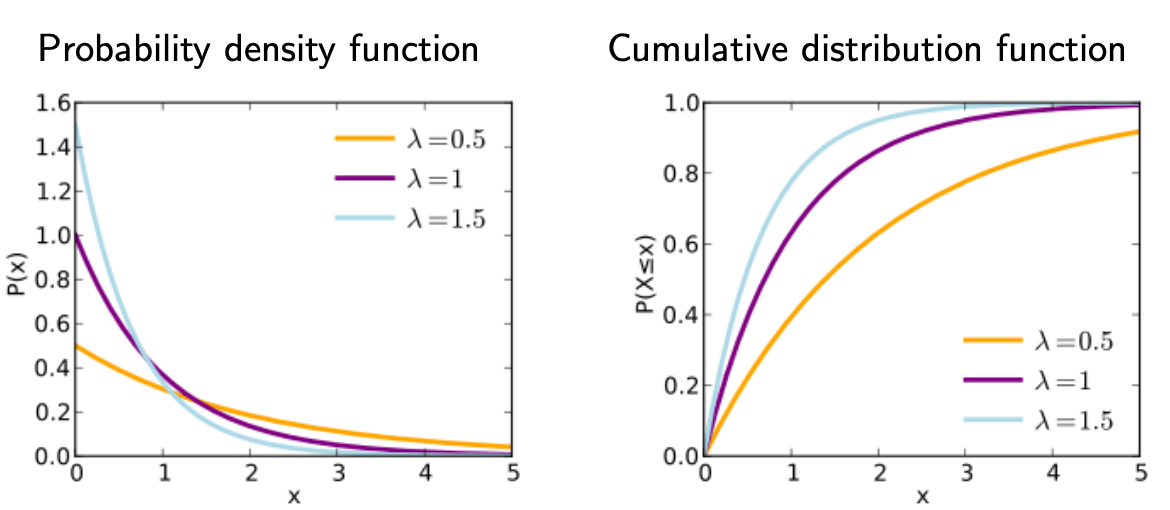
\includegraphics[width=0.8\textwidth]{Images/06 - Stochastic Simulation of Chemical Reactions/Graphs_Density_Cumulative.png}
    \caption{example of a graph for a Density Function and a Cumulative Function} 
\end{figure}

For every reaction in the set of reaction I am considering I have a propensity that is associated to a probability distribution. We can interpret reaction as parallel processes that happen recursively and the frequency of the occurrence are computed by exponential distribution

\subsubsection{Properties of exponential distribution}
There are two important properties of the exponential distribution:
\begin{itemize}
    \item \textbf{The exponential distribution is memoryless:}
        \begin{equation*}
            P(X > t + s | X > s) = P (X > t)
        \end{equation*}
        This allows a simulation algorithm in which the exponential distribution is used to forget about the history of the simulation.

    \item Let $X_{1}, ..., X_{n}$ be some independent exponentially distributed random variables with parameters $\lambda_{1}, ..., \lambda_{n}$, then the equation:
        \begin{equation*}
            X = min(X_{1}, ..., X_{n}
        \end{equation*}
        is also exponentially distributed.
        We set $\lambda = \lambda_{1} + ... + \lambda_{n}$. This allows a simulation algorithm to use a unique exponential distribution for the whole set of reactions to be simulated.    
\end{itemize}

\subsection{Introducing the algorithm}
Given:
\begin{itemize}
    \item A set of molecular species $\{S_{1}, ..., S_{n}\}$.
    \item an initial numbers of molecules of each species $\{X_{1}, .., X_{n}\}$ with $X_{i} in \mathbb{N}$.
    \item a set of chemical reactions $\{R_{1}, ..., R_{M}\}$.
\end{itemize}
Gillespie's algorithm computes a possible evolution of the system.\par
The \textbf{state} of the simulation:

\begin{itemize}
    \item is a vector representing the multiset of molecules in a chemical solution (at the start it is initialized as $[X_{1}, ..., X_{n}]$).
    \item a real variable $t$ representing the simulation time (at the start it is initialized as $t = 0$).
\end{itemize}

Then the algorithm iterates the following steps until it reaches a final value indicated as $t_{stop}$:
\begin{itemize}
    \item  The time $t + \tau$ at which the next reaction will take place. The time is randomly chosen with $\tau$ exponentially distributed with parameter $a_{0} = \sum^{m}_{v=1} a_{v}$
    \item The reaction $R_\mu$ that has to occur at time $t + \tau$ is randomly chosen with probability $\frac{a_{\mu}}{\sum^{M}_{v=1} a_{v}}$
\end{itemize}

At each step t is incremented by $\tau$ and the multiset representing the chemical solution is updated by subtracting reactants and adding products.

\subsection{Implementation details}

\subsubsection{Generation of $\tau$}
Recall that $\tau$ is randomly chosen at each step. A random number with any probability distribution can be computed froma  random number with uniform distribution by applying the \textbf{inversion sampling method}. The idea is to use the inverse of the cumulative distribution function.

Given a cumulative distribution function $F$ of a probability distribution $dist$ and a uniformly  distributed random variable $U$, the variable $X = F^{-1}(U)$ is a random variable with distribution $dist$.\par

In the case of the exponential distribution, the cumulative distribution function for $x \geq 0$ is $F(x) = 1 - e^{- \lambda x}$. Let us now invert the function:

\begin{align*}
    &F(X) = 1 - e^{- \lambda x} \Rightarrow 1 - F(x) = e^{- \lambda x}
    \Rightarrow ln(1 - F(x)) = - \lambda x \\ &\Rightarrow - \frac{1}{\lambda} ln(1 - F(x)) = x \Rightarrow \frac{1}{\lambda} ln \frac{1}{1 - F(x)} = x
\end{align*}

So we obtain:

\begin{equation*}
    F^{-1}(Y) = \frac{1}{\lambda}ln( \frac{1}{1 - Y})
\end{equation*}

Since $Y$ is uniformly distributed, also $1 - Y$ is uniformly distributed. This allows us to simplify the definition of $F^{-1}$ as:

\begin{equation*}
    F^{-1}(Y) = \frac{1}{\lambda}ln( \frac{1}{Y})
\end{equation*}

where:

\begin{itemize}
    \item $\tau$ is exponentially distributed with parameter $a_{0}$ can be computed as $\tau = \frac{1}{a_{0} ln ( \frac{1}{Y})}$ with $Y$ obtained from a standard random number generator.
\end{itemize}

\subsubsection{Choice of reaction $R_{\mu}$}
Recall that $R_\mu$ is the reaction we randomly choose to take action at the step $\tau$. First of all $R_\mu$ will be choose with probability $\frac{a_{\mu}}{a_{0}}$.\par
We do this by following these steps:
\begin{itemize}
    \item We generate a random number $N$ uniformly distributed in $[0, a_{0}$, that is $N = n * a_{0}$ with $n \in [0,1)$ obtained by using a standard number generation.
    \item we start summing $a_{1}, a_{2}, ...$
    \item as soon as the sum becomes greater than $N$, the number of completed iterations gives you $\mu$
\end{itemize}

\begin{figure}[h]
    \centering
    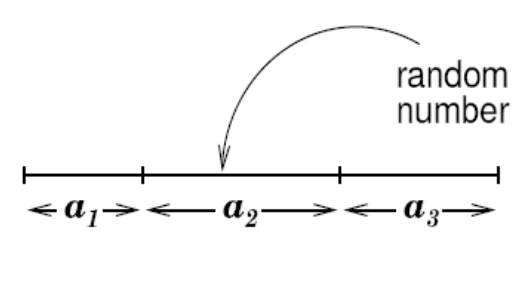
\includegraphics[width=0.5\textwidth]{Images/06 - Stochastic Simulation of Chemical Reactions/Random_Number.png}
    \caption{Choosing the random number} 
\end{figure}

\textbf{Note:} $\mu$ is the smallest integer $k$ satisfying $\sum^{k}_{i=1} a_{i} > na_{0}$ with $n$ uniformly distributed in $[0,1)$

\subsection{Computational cost of Gillespie's algorithm}
The problem of this stochastic approach is the computational cost: because I am executing reaction one by one, I have to repeat the simulation sever time to explore as many behaviour as possible, wasting a lot of time. In the case of large models this may become extremely high, like for example:

\begin{itemize}
    \item when there are large number of molecules
    \item kinetic constant are high
\end{itemize}
In respect to ODEs, this is the only disanvantage.   

\subsection{Variants}
To solve the computational drawback, several variants of Gillespie's algorithm have been introduces.

\subsubsection{Exact approaches}
\textbf{Exact approaches} are variants that improve the computation cost without introducing any approximation:

\begin{itemize}
    \item Gibson and Bruck proposed the use indexed binary tree priority queue to improve the choice of the reaction $R_\mu$ for each step.
    \item Cao et al. and McCollum et al. proposed dynamical ordering strategies for reaction propensities $a_{1}, ...$ in order to probabilistically reduce the time needed to choose $R_\mu$ at each step.
\end{itemize}

\subsubsection{Approximate approaches}
\textbf{Approximate approaches} aims to reduce the computational cost by reducing the number of steps of the overall computation:

\begin{itemize}
    \item Gillespie proposed the $\tau$-leaping method: the idea is to allow several reactions to take place in a single longer time step, under the condition that reaction rates do no change too much during that time.
    \item Gillespie et al. proposed the slow-scale Stochastic Simulation Algorithm ssSSA which separates fast reactions from slow reactions. At each step fast reactions are dealt with by assuming that they reach a dynamic equilibrium, so only their stady state is computed. Slow reaction are simulated one by one in the standard SSA.
    \item Hybrid simulation is a technique which combines ODEs with stochastic simulation: ODEs are applied to molecules occurring in big numbers, stochastic simulation to molecules occurring in small number.
\end{itemize}

\textbf{Note:} the $\tau$-leaping method is the most common.


\chapter{Transition Systems}
We want to start considering models that permit us to \textbf{study the global behaviour of a system}. Assume we are interested in studying whether a system can reach a bad state:
\begin{itemize}
    \item If we use ODEs we can state only the "average" behaviour of a system.
    \item if we us a Stochastic simulator we can only study a number of different possible behaviours.
\end{itemize}
Both approaches does not guarantee that the system will never reach a bad state. To solve this problem we need to introduce a new way of modeling the system behaviour by using Transition Systems.\par
Transition Systems are \textbf{another model of behavior}, so another way to specify how a value changes over time.

\section{What is a Transition System}
A Transition System is a pair $(S, \rightarrow)$ where:
\begin{itemize}
    \item S is a \textbf{set of states}.
    \item $\rightarrow \subseteq S \times S$ is the \textbf{transition relation}.
\end{itemize}
Given two states $s, s^{'} \in S, (s, s^') \in \rightarrow$, then we can write $s \rightarrow s^'$.\par 
If instead we have $s \nrightarrow$ it denotes that there exists no $s^' \in S$ s.t. $s \rightarrow s^'$.\par
Note that:

\begin{itemize}
    \item The set of states can be infinity (typically is assumed to be recursively enumerable).
    \item Transitions describe system state changes.
    \item A state may have more than one outgoing transitions ( $s \rightarrow s^'$ and $s \rightarrow s^{''}$ capturing \textbf{non-deterministic behaviors}. The fact that $s_1$ may evolve in either $s_2$ or $s_3$ does not necessary mean that there is a random choice between the two possibilities. The state choosen could depend froma timer, a scheduler, a probabilistic choice and so on. In general, non-determinis is an \textbf{abstraction} of choice criterion that we simply do not want to model.
\end{itemize}

\section{Trace}
A trace $t$ in a Transition System is a path, meaning a sequence of states t = $s_0, s_1, ..., s_i, s_{i+1}, ...$ such that for each $s_i$ and $s_{i+1}$ ($i \in from the initial state \mathbb{N}$ it holds $s_i \rightarrow s_{i+1}$. $s_0$ is always chose as the \textbf{initial state}.
Note:
\begin{itemize}
    \item t = $s_0$ is the \textbf{minimal trace}.
    \item a trace t is maximal if either t is infinite or $t = s_0, s_1, ..., s_n$ and $s_n \nrightarrow$.
\end{itemize}

\section{Reachability}
Given a state s in a Transition System $(S, \rightarrow)$ we can say that s is reachable if starting from the initial state $s_0$ there exists a trace that starts from $s_0$ and ends at $s$: $t = s_0, s_1, ..., s_n, s$.\par
Very often a Transition System is used to verify that in the model we can reach a particular (good or bad) state.

\par{Class of Transition Systems - Kripke Structures}
A Kirpke Structure is a class of Transion Systems where states are characterized by a set of \textbf{atomic propositions} that can either be true or false. \par
Given a (finite) state of atomic propositions $AP$, a Kripke Structure $K$ is a Transition System $(S, \rightarrow)$ where $S = \mathcal{P}(AP)$.
\begin{itemize}
    \item $\mathcal{P}(AP)$ denotes the powerset of AP.
    \item The interpretation is that an atomic proposition $a$ is contained in a state if and only if it is true in that state
\end{itemize}

\textbf{Note: a state $s$ contains the proposition that are true when inside it.}

\section{Transition Systems over a set of variables}
Given a set of variables $X = \{ X_1, X_2, ..., X_n\}$ and a set of domains $\{D_1, D_2, ..., D_n\}$ s.t. $D_i$ is the domain of $X_i$, a Transition System over X is a Transition System $(S, \rightarrow)$ where $S = D_1 \times D_2 \times ... \times D_n$.

\subsection{Transition Rules}
Given a Transition System over a set of variables, it can be specified b y giving a set of \textbf{transition rules} having the following form:
\begin{center}
    guard $\rightarrow$ update
\end{center}
where:
\begin{itemize}
    \item \textbf{guard}: is \textbf{conjunction of conditions} on the state variables, each having the form $X_i$ op Exp (op is a comparison operator).
    \item \textbf{update}: is a \textbf{conjunction of assignments} to state variables, each having the form $X^{'}_{i} = $ Exp, with $X^{'}_{i}$ denoting the new values of $X_i$ 
\end{itemize}

The idea is that the transition relation contain a transition between each pair of states $s_1, s_2$ s.t.:
\begin{itemize}
    \item $s_1$ satisfies the guard.
    \item  $s_2$ can be obtained by applying to $s_1$ the assignments described in update.
\end{itemize}

%starts Lecture 8%

\section{Labeled Transition Systems}
Consider a Concurrent Interaction Systems where we have several components that are in some extent independent, but they can interact with each other. Representing the system as a whole would be overwhelming, requiring lots of variables and rules. Instead it would be more natural to represent it in a \textbf{Compositional Way} by separating the variables and rules depending of which component they refer to (similar approach to object oriented programming where we create programs that use several classes, but each one is defined separately).\par
In order to define this compositionality feature, we need to find a way to define a transition system based on the individual components, \textbf{taking into account that they could interact between each other}. This means that in the case of two components that interact with each other, when merging their transition systems I should be able to unify their rule that explain the interaction between them. In order to recognize these activities we introduce a \textbf{labels} and define Labeled Transition Systems.\par
Labeled Transition Systems (LTS) are an extended version of Transition Systems in which transitions are enriched with labels. Formally, a LTS is a triple $(S, L, \rightarrow)$ where:
\begin{itemize}
    \item S is a set of \textbf{states}
    \item L is a set of \textbf{labels}
    \item $\rightarrow \subseteq S \times L \times S$ is a \textbf{labeled transition relation}. the triple $(s, \ell, s^{'}) \in L$ is usually denoted as $s \xrightarrow{\ell} s^{'}$. 
\end{itemize}

\subsection{Transition Labels}
Transitions labels $\ell$ describe the action performed by the system (or a single components) during a transition. We distinguish two types of labels:

\begin{itemize}
    \item Labels that use $\tau$ describe an internal action, that is one that is performed in isolation by the single component that contains it.
    \item Other labels ($a, b, c, ...)$ describe potential actions the system (or component) could perform by interaction with some other component.
\end{itemize}

\subsection{Synchronization}
There are two ways to model synchronization:
\begin{itemize}
    \item \textbf{Binary synchronization:} it specify the interaction between two components. A transition with label $a$ of one components has to be performed together with a transition with label $\overline{a}$ (same symbol, but overlined) of another component.

    \item \textbf{Global synchronization:} actions that are synchronized among all system component. All components having a transition with the same label $a$ must perform such a transition together.
\end{itemize}

\textbf{Note:} the synchronization of a number of transitions result in a new $\tau$ transition.
\chapter{Markov Chains}
Sometimes the choice criterion for the transition to pick is probabilistic or due to a stochastic race between poisson processes (race condition). To take care of these cases we need to extend the Transition Systems.

\section{Discrete Time Markov Chains}
Let us extend Transition Systems introducing probabilities.\par
A Discrete Time Markov Chain is a pair $(S, P)$ where:
\begin{itemize}
    \item S is the set of \textbf{states}.
    \item $P: S \times S \rightarrow [0, 1]$ is the \textbf{probability transition matrix} such that for all $s \in S$ in holds:
    \begin{equation*}
        \sum_{s^{'} \in S} P(s, s^{'}) = 1        
    \end{equation*}
\end{itemize}

The probability transition matrix can also be expressed as a \textbf{probabilistic transition relation} $\rightarrow \subseteq S \times [0,1] \times S$ such that $(s, p, s^{'}) \in \rightarrow$ if and only if $P(s, s^{'}) = p > 0$. \par
\textbf{Note:} if $p = 0$ then the transition is usually omitted. \par

When the set of states is finite ( $S = \{s_{0}, s_{1}, ..., s_{n} \} )$ the probability transition matrix can be represented as a square matrix:

\[
P = \begin{bmatrix}
p_{00} & p_{01} & ... & p_{0n} \\
p_{10} & p_{11} & ... & p_{1n} \\
... & ... & ... & ... \\
\vdots & \vdots & ... & \vdots \\
p_{n0} & p_{n1} & ... & p_{nn}
\end{bmatrix}
\]

where $p_{ij} = P(s_{i}, s_{j})$ and the sum of each row is equal to 1. \par

In Discrete Time Markov Chains we usually have a probability distribution of initial states, represent as a vector:
\begin{itemize}
    \item $[1, 0, 0]$ means that state $s_0$ is the only initial state
    \item $[0.5, 0.5, 0]$ means that $s_{0}$ and $s_{1}$ are equally likely to be initial states
\end{itemize}

The constraint $\sum_{s^{'} \in S} P(s, s^{'}) = 1$ implies that every state has at least one outgoing transition (otherwise the sum would be 0), hence deadlocks correspond to states with a self-loop.

\section{Paths}
A path of a Discrete Time Makov Chain (DTMC) is the same concept behind the trace for a Transition System:\par
A path $\pi$ of a DTMC described by the pair $(S, P)$ with initial state $s_{0}$ is a possibly infinite sequence of states $\pi = s_{0}, s_{1}, ...$ such that for each $s_{i+1}$ with $i \in \mathbb{N}$ in $\pi$ it holds $P(s_{i}, s_{i+1}) > 0$.\par

The probability of a path is simply the product of the probabilities of its transitions:
\begin{equation*}
    Prob(s_{0}, s_{1}, ..., s_{n}) = \prod^{n-1}_{i=0} P(s_{i}, s_{i+1})
\end{equation*}
\begin{center}
    or if we do not know where it ends:
\end{center}
\begin{equation*}
    Prob(s_{0}, s_{1}, ...) = \prod_{i \in \mathbb{N}} P(s_{i}, s_{i+1})
\end{equation*}

\section{Probabilistic Reachability}
In a Deterministic Time Markov Chain it is possible to compute the probability that the system will reach a given state:

\begin{itemize}
    \item \textbf{Reachability:} property expressing whether a given state can be reached (there exists a path leading to it).
    \item \textbf{Probabilistic reachability:} probability of reaching a given state (probabilities of all the paths leading to it).
\end{itemize}

Since paths are independent events, their probabilities can be summed.\par
The probability of reaching state s of a DTMC $(S, \rightarrow)$ from the initial state $s_{0}$ is the sum of the probabilities of all paths leading to it. Below the mathematical formula:
\begin{equation*}
    ProbReach(s_{0}, s) = \sum_{\pi \in Reach(s_{0}, s)} Prob(\pi)
\end{equation*}
where $Reach(s_{0}, s)$ is the set of paths reaching s (it can be infinite).

\section{Compute probabilistic reachability}
Solving probabilistic reachability $ProbReach(s, s^{'})$ amounts to solving a system of linear equations in order to obtain $x_{s}^{'}$:
\[
\begin{cases}
    1 \ \ \ \ if \ s_{i} = s^{'} \\
    \sum_{s_{j} \in S} P(s_{i}, s_{j}) X(s_{j}) \ \ \ otherwise
\end{cases}
\]
where P is the probability transition matrix of the DTMC. This can be done by applying iterative computational algebra methods.

\section{Continuous Time Markv Chains (CTMC)}
Now let's extend Transition Systems with stochastic rates:\par
A Continuous Time Markov Chain is a pair $(S, R)$ where:
\begin{itemize}
    \item $S$ is a set of \textbf{states}
    \item $R ; S \times S \rightarrow \mathbb{R}_{\geq {0}}$ is a \textbf{transition rate matrix}
\end{itemize}

The transition rate matrix can be expressed also as a \textbf{stochastic transition relation} $\rightarrow \subseteq S \times \mathbb{R}_{\geq 0} \times S$ s.t. $(s, r, s^{'}) \in \rightarrow$ if and only if $R(s, s^{'} = r > 0$ (if $r = 0$ we omit it).

\subsection{Race conditions}
If we have multiple states $s{'}$ such that $R(s, s^{'}) > 0$ then we can have a \textbf{race condition}, that is the "fastest" transition determines the next state of the system. To be sure which transition we take we first have to resolve two questions,

\subsubsection{How many time we spend in a state before the transition?}
We define the \textbf{exit rate of the state s} $E(s)$ which describes the time I spend to stay in s is exponentially distributed which is the sum of the rate of the outgoing transitions:
\begin{equation*}
    E(s) = \sum_{s^{'} \in S} R(s, s^{'})    
\end{equation*}

\subsubsection{Which transition is eventually taken?}
The choice of the transition to take is proportional to the rate of each transition and is independent from the time at which it occurs.

\subsection{Discrete Time Markov Chain of a Continuous Time Markov Chain}
Since we can ignore time when deciding which transition to take, we can use a Discrete Time Markov Chain to model it. We obtain our DTMC by normalizing the transition rates of the Continuous Time Markov Chain we have, in respect to the exit rate of each state.
So given a $CTMC (S, R)$, its embedded DTMC is the $DTMC (S, P)$ where for any $s, s^{'} \in S$:
\[
P(s,s^{'}) =
\begin{cases}
    R(s, s^{'})/E(s) \ \ \ if \ \  E(s)>0\\\
    1 \ \ \ \ \ if \ \ E(s) = 0 \And s = s^{'}\\\
    0 \ \ \ \ \ otherwise
\end{cases}
\]

\section{Uniformised DTMC}
Given a CTMC, what is the probability of the system to be in a state $s$ at a given time? To solve this we introduce the uniformised DTMC.\par
The idea is that I choose a normalization factor called the \textbf{uniformisation rate} $q$ which is not the \textbf{exit rate of each state}, but a single factor for all parameters. The uniformisation rate q is set as being greater or equal to all the exit rates of the CTMC rates. Then I construct the uniformised DTMC by recompute each rate r of the CTMC discretizing them into probability $\frac{r}{q}$. Self-loops are added where necessary.

\subsection{Interpretation of the uniformised DTCM}

\begin{itemize}
    \item a transition in the uniformised DTMC describes a step with duration $\frac{1}{q}$
    \item q should be chosed big enough to assume that at most one transition can occur during a $\frac{1}{q}$ time interval
\end{itemize}

Transient probabilistic reachability of a CTMC can now be computed as probabilistic reachability in the uniformised DTMC, bu taking the length of the paths in the DTMC into account.
\chapter{Model Checking}
Model Checkers are tools specialized in answering question in regard to system we want to analyze. \par

\section{Non-deterministic setting}
\textbf{Assume we are in a non deterministic setting}: the system is described by using a transition system and question we want answered are modeled using temporal logic specification (a set of logic formulas). Given this parameters the model checker visit the transition system according to the logic formulas and verify if the question is true or false. If the question is false it returns a \textbf{counter-example}.

\section{Deterministic setting}
If I have a probability distribution associated to the transition system, then I can extend the approach by instead of checking the satisfiability of a boolean formula, I compute the probability that a formula is satisfied.

\section{Problems with this approach}
The larger the transition system, the more and more become complex; the larger the boolean formulas the more complex the analysis to check its satisfiability. In the end all of our study will amout in checking reachability probability properties.

\section{Logic in Non-deterministic system}

\section{Computation Tree Logic}
Computation Tree Logic (CTL) is one of the main logic for expressing requirements on behaviours. In CTL we can write formulas that can be true or false. 

\subsection{Syntax}
Formulas can be declare for states or paths:
\begin{itemize}
    \item \textbf{State formulae:}
        \begin{itemize}
            \item $\phi ::= true | a | \phi \land \phi | \lnot \phi | A \psi | E \psi$
            \item $a$ is an atomic proposition.
            \item $\psi$ is a path formula.
        \end{itemize}

    \item \textbf{Path formulae:}
        \begin{itemize}
            \item $\psi ::= X \phi | F \phi | G\phi | \phi U \phi$
            \item \textbf{F:} for "future" states will satisfy the condition
            \item \textbf{G:} for "global" states (all the ones considered) will satisfy the condition.
            \item \textbf{U:} for "until" a condition, another condition must be satisfied.
        \end{itemize}
\end{itemize}

\subsection{Semantics}

\begin{itemize}
    \item \textbf{Quantifiers:}
        \begin{itemize}
            \item \textbf{A:} universal quantifier (any).
            \item \textbf{E:} existential quantifier (exists).
        \end{itemize}
    \item \textbf{Temporal operators:}
        \begin{itemize}
            \item \textbf{F:} the future states
            \item \textbf{G:} the global states.
            \item \textbf{U:} until, it asks if a certain property is true UNTIL another property kicks in.
        \end{itemize}
\end{itemize}

%Immagine pag 7 slile 04-prob logics.ppt%

\section{Probabilistic Computation Tree Logic}
Is an extension of CTL that takes intro account probability distribution.

\subsection{Syntax}
The main difference is that in state formulas we change the quantifiers with \textbf{probabilistic quantifiers}. Instead of asking if a formula is true for all states or for some, we ask if the probability that a certain condition is true is $\geq$ than a given probability.
\begin{itemize}
    \item \textbf{State formulae:}
        \begin{itemize}
            \item $\phi ::= true | a | \phi \land \phi | \lnot \phi | P_{~p} [\psi]$
            \item $a$ is an atomic proposition
            \item $p \in [0,1]$ is a probability bound
            \item $~ \in \{<, >, \leq, \geq \}$
        \end{itemize}
    \item \textbf{Path formulae}
        \begin{itemize}
            \item $\psi ::= X \phi | \phi U^{\leq k} \phi | \phi U \phi$
            \item \textbf{X:} stands for "next"
            \item $U^{\leq k}$: stands for "bounded until"
            \item \textbf{U:} stands for "until"
            \item $k \in \mathbb{N}$
        \end{itemize}
\end{itemize}

\chapter{Multiset Rewriting and P Systems}
A formal specification of chemical reaction and of their behavior can be given in terms of \textbf{MultiSet Rewriting (MSR)}.\par

\section{Multiset}
With \textbf{multiset} we intend a variant of the mathematical notion of set in which elements can be repeated. In this way we can interpret chemical solution as multisets representing molecules.

\subsection{Formalizing multisets}
Given a (finite or infinite) support set $\Sigma$, we methematically represent a multiset M over $\Sigma$ in two ways:
\begin{itemize}
    \item \textbf{set of pairs:} $M \subseteq \Sigma \times \mathbb{N}$
    \item \textbf{ mapping:} $M: \Sigma \rightarrow \mathbb{N}$
\end{itemize}

\subsubsection{Example}
Given the set $\Sigma = \{A, B, C\}$ and the multiset $M = \{A, A, A, B, B, C, C, C \}$ over $\Sigma$ can be represented in two ways:

\begin{itemize}
    \item \textbf{set of pairs:} $M = \{ (A, 3), (B, 2), (C, 3) \}$
    \item \textbf{mapping:} $M(A) = 3, M(B) = 2, M(C) = 3$
\end{itemize}

\textbf{Note:} these representations actually correspond to the representation of chemical solutions we considered in PRISM.

\subsection{Representing Multisets as strings}
Another useful representation of multisets that is very similar to formal grammars is a \textbf{string}.\par
We interpret the set $\Sigma$ as an \textbf{alphabet}, and the multiset $M$ over $\Sigma$ correspond to strings over such alphabet. Note that in a string representing a multiset, \textbf{the order of the symbols does not matter}, so string permutations result in equivalent representation.

\subsubsection{Example}
Given $\Sigma = \{A, B, C\}$ and the multiset $M = \{(A, 3), (B,2), (C,3)\}$ we can represent M as the string:
$M = AAABBCCC = A^{3}B^{2}C^{3}$ and all its possible permutations.\par
Multiset union can be expressed as string concatenation:
\begin{equation*}
\{(A,3), (B,2), (C,3) \} \cup \{ (A,2), (B,1)\} = \{(A,5), (B,3), (C,3)\} = A^{5}B^{3}C{3}    
\end{equation*}

\section{Representing reactions as rewriting rules}
Rules are similar to rules in a formal grammar:\par
A multiset rewriting rule is a pair $(u, v)$ with $u, v \in \Sigma^{*}$ usually denoted as $\mapsto$. When we apply the rule $(u,v)$ to a multiset $w \in \Sigma^{*}$ s.t. $u \subseteq w$ what we obtain is the multiset in which \textbf{$u$ as been replaced by $v$}

\section{Definition of MultiSet Rewriting System}
A MultiSet Rewriting System (MSRS) is a pair $S = < \Sigma, \mathcal{R} >$ where $\Sigma$ is the \textbf{alphabet of symbols} and  $\mathcal{R}$ is a \textbf{set of multiset rewriting rules}.\par
Given a multiset in $\Sigma^{*}$ we can use the mechanism of rewriting rule application to compute \textbf{traces} of the multiset rewriting system.

\section{Interleaving semantics}
The behavior of a MSR system can also be described as a Transition System: we can define an (interleaving) semantics for MSR defining inference rules incorporating the mechanism of rewriting rule application.\par
The interleaving semantics of a MSR system $< \Sigma, \mathcal{R}>$ is the Transition System ${\Sigma^{*}, \rightarrow}$ where $\rightarrow \subseteq \Sigma^{*} \times \Sigma^{*}$ is the least transition relation satisfying the following inference rule:
\begin{equation*}
    \frac{u \mapsto v \in \mathcal{R}}{uw \mapsto vw}
\end{equation*}

\section{Stochastic MSR}
We can extend the stochastic syntax and semantics of MSR to incorporate stochastic rates.\par
Given an alphabet $\Sigma$ a stochastic multiset rewriting rule is a tuple $(u, v, r)$ where $u, v \in \Sigma^{*}$ and $r \in \mathbb{R}^{+}$, usually denoted $u \mapsto^{r} v$

\subsubsection{Stochastic Multiset Rewriting System}
A Stochastic MSR system is a pair $S = <\Sigma, \mathcal{R}>$ where $\Sigma$ is an alphabet of symbols and $\mathcal{R}$ is a set of stochastic multiset rewriting rules.

\subsubsection{Semantics of Stochastic MSR}
The semantics of a stochastic MSR system is a Continuous Time Markov Chain $(\Sigma^{*}, \rightarrow)$ where $\rightarrow \subseteq \sum^{*} \times \mathbb{R}^{+} \times \sigma^{*}$ is the least stochastic transition relation satisfying the following inference rule:
\begin{equation*}
    \frac{ u \mapsto^{r} v \in \mathcal{R}}{uw \xrightarrow{r \cdot f(u, uw)} vw}
\end{equation*}

Where $f(u, uw)$ gives the number of instances of $u$ in $uw$.

\section{Introducing parallelism}
We can defines variantas of the language, in particular regarding the introduction if prarallelism in the application of rewriting rules:
\begin{itemize}
    \item \textbf{simple parallelism:} one or more rule are applied at each step.
    \item \textbf{maximal parallelism:} as many rules as possible are applied at each step.
\end{itemize}
In this way we can model classes of systems where there are simultaneous events. In particular we are interested in maximal parallelism because its models system where there is a strong formal synchronization.

\subsection{Parallel semantics of MSR}
The parallel semantics of a MSR system $<\Sigma, \mathcal{R}>$ is the transition system $(\Sigma^{*}, \rightarrow)$ where $\rightarrow \subseteq \sum^{*} \times \sum^{*}$ is the lest transition relation satisfying the following inference rules:

\begin{equation*}
    \frac{u \mapsto v \in \mathcal{R}}{u \rightarrow v}
\end{equation*}

\begin{equation*}
    \frac{w_{1} \rightarrow w^{'}_{1} \ \ \ w_{2} \rightarrow w^{'}_{2}}{w_{1}w_{2} \rightarrow w^{'}_{1}w^{'}_{2}} 
\end{equation*}

\begin{equation*}
    \frac{w \rightarrow w^{'} \ \ \ u \nrightarrow}{wu \Rightarrow w^{'}{u}} 
\end{equation*}

\section{Multiset languages}
A language where we ignore the sequential ordering of symbols in its words becomes a \textbf{multiset language}. A multiset language is a set of multisets of terminal symbols and is generated by a multiset grammar.\par
This change in the representation of the language causes a significant change in the expressiveness of the languages, becoming more weak. Multiset languages can run on a weak-Turing Machine.

\subsection{Introducing maximal parallelism in multiset languages}
The maximal parallelism re-introduce the expressive power of grammars I lost using multiset languages. General multiset grammar rules applied with maximal parallelism are again able to generate any recursively enumerable language. Having a more complex grammar requires a Turing-complete form of automaton to accept a string from it.

\section{P Systems}
P Systems is a variant of Multiset rewriting with maximal parallelism (P stands for Paul which is the name of the inventor). What set apart P Systems from normal Multiset rewriting is that it has more than one multiset in the set.\par
The key elements of P Systems are:
\begin{itemize}
    \item \textbf{Membranes:} they creates compartments used to distribute computations.
    \item \textbf{Multisets:} abstraction of chemical solutions that are used as data.
    \item \textbf{Evolution (rewriting) rules:} abstraction of chemical reaction that are used as programs.
\end{itemize}

\begin{figure}[h]
    \centering
    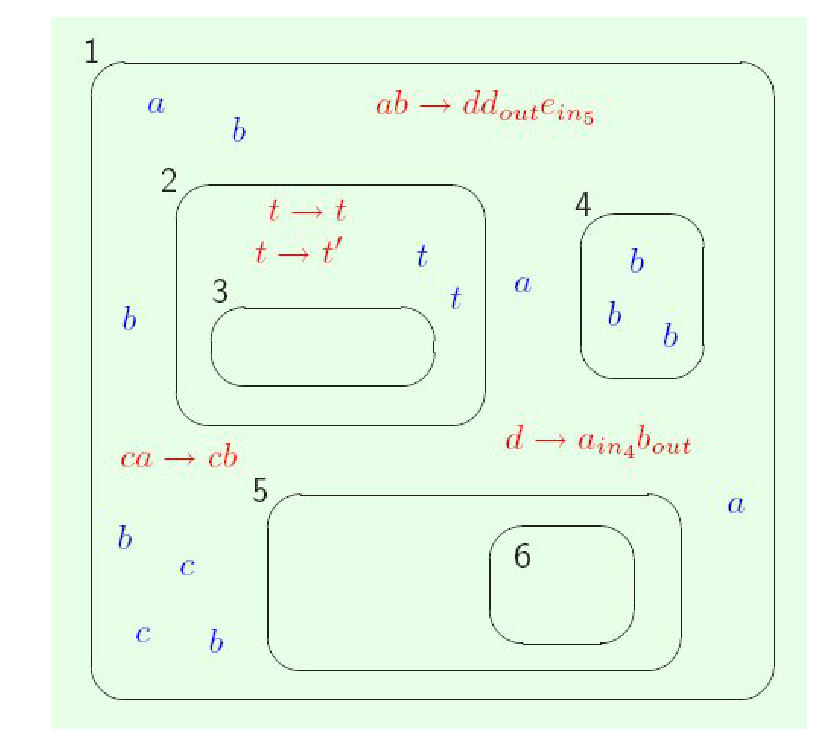
\includegraphics[width=0.5\textwidth]{Images/11-Multiset Rewriting and P Systems/PSystem.png}
    \caption{Example of a P System} 
\end{figure}

\subsection{Formal definition of a P System}
A P System $\Pi$ is given by:
\begin{equation*}
    \Pi = (V, \mu, w_{1}, ..., w_{n}, R_{1}, ..., R_{n})
\end{equation*}

where:
\begin{itemize}
    \item \textbf{V:} is an alphabet whose elements are called objects.
    \item $\mu \subset \mathbb{N} \times \mathbb{N}$ is a membrane structure, s.t. $(i, j) \in \mu$ denotes that the membrane labeled by $j$ is contained in the membrane labeled by $i$.
    \item $w_{i}$ with $1 \leq i \leq n$ are strings from $V^{*}$ representing multisets over V associated with the membranes $1, 2, ..., n$ of $\mu$.
    \item $R_i$ with $1 \leq i \leq n$ are finite sets of evolution rules associated with the membranes $1, 2, ..., n$ of $\mu$.
\end{itemize}

\subsection{Evolution rules}
An evolution rule in the form $u \rightarrow v$ consists of a multiset of objects $u$ (representing reactants) and a multised of messages $v$ (representing products). A message may have one of the following forms:
\begin{itemize}
    \item $a_{here}$: means that object $a$ remains in the same membrane. Often we omit $here$ and just leave $a$ alone.
    \item $a_{out}$: means that object $a$ is sent out of the membrane.
    \item $a_{in}$: means that object $a$ is sent into the child membrane I.
\end{itemize}

Evolution rules are classified in two ways:
\begin{itemize}
    \item \textbf{non-cooperative rules:} the left-hand side consists of a single object (e.g. $a \rightarrow b^{2}d_{out}$)
    \item \textbf{cooperative rules:} the left-hand side can be any multiset of objects (e.g. $a^{2}b \rightarrow b^{2}d_{out}$). A particular case of cooperative rules are catalytic rules, namely rules of the form $ca \rightarrow cb^{2}$ where $c$ belongs to a special set of objects called catalyst.
\end{itemize}

\subsection{Downsides of P Systems}
Programming P Systems is very difficult since evolution rules are very basic.\par
For this reason over the years have been proposed variants of P Systems, obtained by considering different types of evolution rules:
\begin{itemize}
    \item with rule priorities.
    \item with promotes and inhibitors.
    \item with dissolution of membranes.
    \item symport/antiport rules.
    \item with active membranes 
    \item and so on...
\end{itemize}
\chapter{Petri Nets}
Petri Nets is a modeling languages notation that allow us to apply different analysis approaches. Petri nets have been proposed to model concurrent systems. 

\section{Concurrent Systems}
A concurrent system is a system (not strictly from computer science) where there are processes of any type executed at any time. In this system you have a workflow where some processes works in parallel (independent from each other) and others work sequentially (they must wait for the previous machines to finish).\par

Petri Nets are a graphical model notation for concurrent systems in which you construct a graph that describe resources and events involving those resources. There are two types of nodes:

\begin{itemize}
    \item \textbf{Places:} represent type of resources. 
        \begin{itemize}
            \item \textbf{Tokens:} represent instances of a resource of some specific type. Tokes stay inside places. The place where they are describe their type
        \end{itemize}
    \item \textbf{Transition:} represent events that change the state of one or more resources. They connect places to places (like a Multiset Rewriting rule or a chemical reaction). Incoming edges are connected to places that provide resources (tokens) that are consumed by the transition, while output edges represent places for which resources have been produced.
\end{itemize}

\section{Firing a transition}
Firing a transition means \textbf{executing it}. In order to fire a transition you must have enough resources in input, then it will produce the necessary resources for the output places.

\section{Formal definition of Petri Nets}
A Petri Net is a tuple $<P, T>$ where:
\begin{itemize}
    \item $P$ is the (finite) set of \textbf{places}.
    \item $T$ is the (finite) set of \textbf{transitions} s.t. each transition $t$ is a tuple $<I, O>$ where:
        \begin{itemize}
            \item $I$ is a function s.t. $t$ consumes $I(p)$ tokens in each place $p$.
            \item $O$ is a function s.t. $t$ produces $O(p)$ tokens in each place $p$.
        \end{itemize}
\end{itemize}

\subsection{Markings}
Tokens that are placed in the network represent\textbf{ the state of the network}. The state of the Petri Net is also called the \textbf{marking of the Petri Net}. A marking con be seen in two different ways:

\begin{itemize}
    \item a function $m$ s.t. $m(p)$ is the number of tokens in place $p$.
    \item a vector $m = <m_{1}, m_{2}, ..., m_{n}$ where $m_{i}$ is the number of tokens in place $p_{i}$. 
    \item a vector $m = <d_{1}p_{1}, ..., d_{n}p_{n}$ where $d_{i}$ represents the number of tokens in $p_{i}$.
\end{itemize}

\subsection{Firing a transition}
Given a transition $t = <I, O>$, it can be fired from $m$ $iff$ for any place p:

\begin{equation*}
    m(p) \geq l(p)
\end{equation*}

If the condition is satisfied then the firing transforms the marking $m$ into a marking $m^{'}$ s.t. for any place p:
\begin{equation*}
    m^{'}(p) = m(p) - I(p) + O(p)
\end{equation*}

This transformation can be described by the following notations:
\begin{itemize}
    \item $m \rightarrow m^{'}$
    \item $Post(m) = \{m^{'} | m \rightarrow m^{'}\}$. $Post(m)$ is the set of markings that can be obtained by firing transitions from $m$ ($Post$ correspond to the transition relation in the Transition Systems)
\end{itemize}

\subsubsection{Initial marking}
The marking that we consider to be the first one is colled the \textbf{initial marking} $m_{0}$.

\subsubsection{Reachable markings}
Given two markings $m$ and $m{'}$ s.t.:
\begin{equation*}
    m \rightarrow m_{1} \rightarrow m_{2} \rightarrow ... \rightarrow m^{'}
\end{equation*}
Then we can say that $m^{'}$ is reachable from $m$.\par
Given the Petri Net $N$ with initial marking $m_{0}$, then the function $Reach(N)$ is the set of reachable markings of N s.t.:
\begin{center}
    Reach(N) = \{$m$ reachable from $m_{0}$\}
\end{center}

\subsection{Ordering on markings}
Markings can be compared using the precedence relation $\preceq$:
\begin{itemize}
    \item $m \preceq m^{'} \iff \forall p. m(p) \leq m^{'}(p)$.
    \item $m \prec m^{'} \iff m \preceq m^{'} \land m \neq m^{'}$
\end{itemize}

\section{What can we use Petri Nets for}
The question we can investigate on Petri Nets are these:
\begin{itemize}
    \item \textbf{Boundedness:} is the number of reachable markings bounded?
    \item \textbf{Place boundedness:} in each place the number of tokens I can obtain is bounded or can it grows in an unbounded way?
    \item \textbf{Semi-liveness:} the transition that are present in a Petri Net will they all be fired? There are some transition that can never be fired?
    \item \textbf{Coverability}
\end{itemize}

\section{Decidability of a marking}
The reachability graph of a Petri Net (aka the Transition System of a MultiSet Rewriting system) can be infinite, \textbf{but the reachability property is decidable}. The computation of decidability has been proven to require \textbf{exponential time}. This means that Petri Net are not Turing equivalent.\par
In order to compute reachability in an efficient way, several alternatived have been proposed:

\subsubsection{Solution 1}
We consider overapproximations of the set of reachable states (based on Place Invariants or on Karp and Miller tree). We compute in polynomial time a set which is an overapproximation of the set of reachable marking. So our solution will include surely ALL the reachable marking, but also it can contain some unreachable ones. So we are only sure that if a marking is not in the overapproximation, then it is not reachable.

\subsubsection{Solution 2}
Instead of consider reachability, we will answer coverability: "is a marking greater or equal than is reachable?" The problem of coverability is weaker than reachability, but easy to compute and meaningful in the context of Petri Nets.

\section{Place Invariants}
Place Invariants are a way to reason about marking which has some analogy which the mass conservation invariant (matter can never be created or destroyed). This can be used to put constraint on a set of reachable markings.\par
Formally a Place invariant (or p-semiflow) is a vector $i$ of natural numbers s.t. for any reachable marking m:
\begin{equation*}
    \sum_{p \in P} i(p) \times m(p) = \sum_{p \in P} i(p) \times m_{0}(p)
\end{equation*}

\subsection{Invariants as overapproximations}
Given a marking $m$ and an invariant $i$, we can say that if $m$ is reachable and $i$ is an invariant, then:
\begin{equation*}
    \sum_{p \in P} i(p) \times m(p) = \sum_{p \in P} i(p) \times m_{0}(p)
\end{equation*}
The reverse is not true.

\subsubsection{Theorem}
$\forall$ Petri Net N:
\begin{center}
    $Reach (N) \subseteq \{ m | m $ respects some invariant of $N\}$
\end{center}

So if a marking does not respect the invariant, \textbf{then we surely know that is not reachable}.

\subsubsection{Theorem: place invariant and boundedness}
If there exists a place invariant $i$ and a place $p$ s.t. $i(p) > 0$, then $p$ is bounded. \textbf{The reverse is not true.}

\section{How to compute Place invariants}
\subsection{Matrix chatacterisation}
Let us represent the Petri Net as a matrix where we but places on the rows and transitions on the cons. We construct a matrix that describes the input tokens that are consumed for a given transition and a matrix for those that have been produced:

\subsubsection{Consumption Matrix}
\[
W^{-} =
\begin{bmatrix}
    I_{1}(p_{1}) & I_{2}(p_{1}) & ... & I_{k}(p_{1}) \\
    I_{1}(p_{2}) & I_{2}(p_{2}) & ... & I_{k}(p_{2}) \\
    \vdots & \vdots & ... & \vdots \\
    I_{1}(p_{n}) & I_{2}(p_{n}) & ... & I_{k}(p_{n})
\end{bmatrix}
\]

\subsubsection{Production Matrix}
\[
W^{+} =
\begin{bmatrix}
    O_{1}(p_{1}) & O_{2}(p_{1}) & ... & O_{k}(p_{1}) \\
    O_{1}(p_{2}) & O_{2}(p_{2}) & ... & O_{k}(p_{2}) \\
    \vdots & \vdots & ... & \vdots \\
    O_{1}(p_{n}) & O_{2}(p_{n}) & ... & O_{k}(p_{n})
\end{bmatrix}
\]

\subsubsection{Incidence Matrix}
We then define the \textbf{incidence matrix} W that represent the global effect of every transition:

\begin{equation*}
    W = W^{+} - W^{-}
\end{equation*}

\section{Computing place invariants}
We have said that place invariants represent mass conservation, so all the reachable markings will preserve that constraint. Reachable markings are obtained by firing transition. Then every transition that fires has to preserve the overall weight of the matrix.\par
Then the weight of the tokens that are produced has to be the same as the weight of the tokens that are consumed in order to preserve the overall weight.\par
So I express invariant by focusing on individual transitions:\par
$\forall$ transition $t = <I, O>$ we should have:
\begin{equation*}
    \sum_{p \in P} I(p) \times i(p) = \sum_{p \in P}O(p) \times i(p)
\end{equation*}

which is the same as putting:
\begin{equation*}
    \sum_{p \in P} (O(p) - I(p)) \times i(p) = 0
\end{equation*}

Now considering the incidence matrix $W$ we have defined previously, any solution $i$ is a place invariant if satisfy the following scalar product:
\begin{equation*}
    i \times W = 0
\end{equation*}

\chapter{Discrete-Event Simulations (DES)}

Discrete Event Simulation is a generalization of the Simulation we have seen so far. Consider the Stochastic Simulations (e.g. Gillespie's algorithm and PRISM), their limitations lies if the events of a system could be not instantaneous. Considers the case when the frequency of events follow different distributions (e.g. fixed delay, uniform distribution within an interval, ...), in that case we need to generalize the simulation to be able to allow these timing issues in our system. \par

Discrete Event Simulation (DES) does not rely on the memory-less property of Stochastic Simulations, \textbf{we have to keep track of what is going on in our system}. DES implement an \textbf{event list} to be aware of the time passing. In an event list we have:

\begin{itemize}
    \item \textbf{State:} is a description of system configuration in terms of a set of variables.
    \item \textbf{Activity:} is a process that involves a sequence of updates of the state variables (events) over time. It has a \textbf{duration}.
    \item \textbf{Event:} is an instantaneous update of the state variables. They can correspond to the start and end of an activity.
    \item \textbf{Event notice:} is a description of a future event with the time at which it will happen.
    \item \textbf{Future Event List:} is a list of event notices ordered by time.
\end{itemize}

%immagine lezione #14 in pag 10/19%

\section{Future Event List}
the Future Event List (FEL) is the queue we have to schedule the future events. It contains notices of all future events that are scheduled and is ordered by increasing time of event notice.\par

%immagine lezione #14 in pag 11/19%

\subsubsection{Generalization of the simulation algorithm using the FEL}
\begin{itemize}
    \item initialize state variables, the FEL and a \textbf{global clock variable} $T = 0$
    \item at each step:
        \begin{itemize}
            \item remove the first event notice $(t, Event)$.
            \item handle Event. This could cause the update of state variables, adding one or more event notices to the FEL and removing one or more scheduled events from the FEL.
            \item update the global cloc $T = t$
        \end{itemize}

    \item we stop when the clock reach a stop time $T_{stop}$ s.t. $T = T_{stop}$ or the FEL is empty. 
\end{itemize}

\subsection{Conditional and Primary Events}
To handle events that have to wait for a condition in ordered to be enable we need to divide events in two types:

\begin{itemize}
    \item \textbf{Primary events:} events whose occurrence in scheduled at a certain time.
    \item \textbf{Conditional events:} events that are triggered by a certain condition becoming true. \textbf{Conditional events are untimed}. For this reason we can store Conditional events at the beginning of the FEL or in an apposite data structure.
\end{itemize}

\subsection{Revised Simulation Algorithm}
We rewrite the simulation algorithm taking into account the two types of events possible:
\begin{itemize}
    \item Initialize variables, FEL and T
    \item Iterate:
        \begin{itemize}
            \item If there is a conditional event enabled, remove and process it (To does not change), otherwise remove and process the first primary event. Finally update T
        \end{itemize}
    \item Continue until the global clock reaches the time stop $T = T_{stop}$ or the Future Event List is empty 
\end{itemize}


\chapter{Cellular Automata}
Agent-Based Modeling is a modeling approach in which system components are represented as agents able to take decisions, perform actions, and interact with other agents or/and the environment.\par
Usually the behaviors of an agent are specified using a high-level programming language.\par
Agent-Based Simulation is a form of Discrete Event Simulation that consists in "executing" agents concurrently.

\section{Considering the environment}
Agents can move in a 2D or 3D environment. Agent position and spatial charateristics of the environment will influence the system dynamics (e.g. agents can only interaction with neighbours; there could be obstacles; resources are distributed across the environment; areas could have different charateristics).

\section{Cellular Automata}
Cellular Automata (CA) allow to describe environments in 1D, 2D or 3D. The environment is described as a matrix of cells. Each cell is defined by its own state that can change by means of rules. Cellular Automata can be used to model Complex Systems with spacial structure.\par

\subsubsection{Multicellularity}
Cellular Automata uses as reference multicellularity ad a way to build complex living systems.\par
Multicellular systems are composed by many copies of cell, our unique fundamental unit. Cells will interact with the ones in his proximity, influencing the fate and behavior of each cell. The result is an heterogeneous system composed by differentiated cells that act as specialized units, even if they all contain the same genetic material and have essentially the same structure.

\section{Modelling cellular systems}


\nocite{*}
\bibliographystyle{plain}
\clearpage\bibliography{bibliography}

\end{document}